\chapter{Riemann Integration}
\chaptermark{Riemann Integration}
\label{ch:riemann}

This chapter answers four related questions:
\[
\boxed{
\begin{array}{c}
\text{When does an integral exist?}\\
\text{How do we compute it?}\\
\text{Why do the familiar calculus rules work?}\\
\text{Where does the Riemann theory begin to break down?}
\end{array}}
\]
Most functions in ordinary calculus are assembled from elementary functions
by algebraic operations and composition. On their natural domains they are
usually very regular---often \(C^\infty\), and therefore continuous---so the
existence hypotheses for proper integrals can become nearly invisible.
Continuity on a compact interval, not continuous differentiability, is already
enough for Riemann integrability. At the same time,
\[
\boxed{\text{elementary formula}\ne\text{automatic global regularity}.}
\]
The functions
\[
1/x,
\]
 \(\log x\), \(\sqrt{x}\), \(\tan x\), and

\[
1/\sqrt{1-x^2}
\]
 all demand attention to their domains and singularities.
Accordingly, existence is checked before computation throughout the chapter.

\section{Partitions and Riemann Sums}

Integration formalizes approximation of accumulated quantities by finite
sums.  Darboux upper and lower sums avoid choosing sample points: they record
the best guaranteed under- and over-approximations on every subinterval.

\begin{definition}[Partition]
Let $a<b$. A \textbf{partition} of $[a,b]$ is a finite ordered set
\[
P=\set{x_0,x_1,\ldots,x_n}
\]
with $a=x_0<x_1<\cdots<x_n=b$. Its mesh is
\[
\operatorname{mesh}(P)=\max_{1\leq i\leq n}(x_i-x_{i-1}).
\]
\end{definition}
Thus $\operatorname{mesh}(P)<\delta$ means that every cell has width less
than $\delta$. Refinement cannot increase mesh. Equal partitions $P_N$
satisfy
\[
\operatorname{mesh}(P_N)=\frac{b-a}{N}\longrightarrow0,
\]
so arbitrarily fine partitions exist.

\begin{definition}[Interval oscillation]
For a bounded function $f$ on a nonempty interval $I$, define
\[
\operatorname{osc}_I(f)=\sup_I f-\inf_I f.
\]
This is the largest possible vertical variation of $f$ on $I$:
\[
\boxed{\operatorname{osc}_I(f)=\sup_{x,y\in I}|f(x)-f(y)|.}
\]
\end{definition}
Indeed, every difference is at most $\sup_I f-\inf_I f$. Conversely, for
each $\eta>0$, choose $x,y\in I$ with
\[
f(x)>\sup_I f-\eta/2,
\qquad
f(y)<\inf_I f+\eta/2.
\]
Then $|f(x)-f(y)|>\operatorname{osc}_I(f)-\eta$, so taking the supremum
proves the reverse inequality without assuming extrema are attained.
Restriction can only reduce the available pairs, and hence
\[
J\subseteq I\Longrightarrow\operatorname{osc}_J(f)
\leq\operatorname{osc}_I(f).
\]
Also $\operatorname{osc}_I(f)=0$ exactly when $f$ is constant on $I$.

\begin{definition}[Upper and lower sums]
Let $f:[a,b]\to\R$ be bounded and let $P$ be a partition. Put
\[
I_i=[x_{i-1},x_i],\qquad \Delta x_i=x_i-x_{i-1},
\]
and
\[
M_i=\sup\set{f(x):x\in[x_{i-1},x_i]},
\qquad
m_i=\inf\set{f(x):x\in[x_{i-1},x_i]}.
\]
The \textbf{upper sum} and \textbf{lower sum} are
\[
U(f,P)=\sum_{i=1}^{n}M_i\Delta x_i,
\qquad
L(f,P)=\sum_{i=1}^{n}m_i\Delta x_i.
\]
\end{definition}

The two panels of Figure~\ref{fig:darboux-sums} use the same function
and partition. The excess height on cell $I_i$ is its oscillation
$M_i-m_i$, so, writing $\Delta x_i=x_i-x_{i-1}$,
\[
\boxed{U(f,P)-L(f,P)=\sum_i
\underbrace{\operatorname{osc}_{I_i}(f)}_{\text{vertical uncertainty}}
\underbrace{\Delta x_i}_{\text{horizontal width}}.}
\]
This cellwise quantity is distinct from the pointwise oscillation introduced
in section~9.6. It organizes the next several estimates: uniform continuity
makes every cell's oscillation small when the partition intervals are short.
\begin{figure}[htbp]
\centering
\begin{tikzpicture}[font=\small,>=Stealth,x=1.15cm,y=1.15cm]
\foreach \shift/\title/\upper in {0/Lower sums/0,6/Upper sums/1}{
\begin{scope}[xshift=\shift cm]
\node at (2,2.7) {\title};
\foreach \i in {0,...,4}{
\pgfmathsetmacro{\a}{.8*\i}
\pgfmathsetmacro{\b}{.8*(\i+1)}
\pgfmathsetmacro{\h}{.35+.1*(\a+.8*\upper)^2}
\filldraw[fill=blue!14,draw=blue!65!black] (\a,0) rectangle (\b,\h);
}
\draw[->] (-.1,0)--(4.35,0) node[right] {$x$};
\draw[->] (0,0)--(0,2.4);
\draw[thick] plot[domain=0:4,samples=60] (\x,{.35+.1*\x*\x});
\node[above left] at (3.9,1.95) {$f$};
\node[below] at (0,0) {$a$};\node[below] at (4,0) {$b$};
\end{scope}}
\begin{scope}[xshift=6cm]
\draw[orange!85!black,thick,<->] (4.25,1.374)--(4.25,1.95)
 node[midway,right,font=\footnotesize] {$M_i-m_i$};
\draw[dashed] (3.2,1.374)--(4.25,1.374);
\draw[dashed] (4,1.95)--(4.25,1.95);
\draw[<->] (3.2,-.55)--(4,-.55) node[midway,below] {$\Delta x_i$};
\end{scope}
\end{tikzpicture}
\caption{The same increasing function and partition give lower rectangles
on the left and upper rectangles on the right. On the marked cell, the
extra area is $(M_i-m_i)\Delta x_i$. Summing these cellwise gaps gives
$U(f,P)-L(f,P)$; small oscillation makes the total gap small.}
\label{fig:darboux-sums}
\end{figure}


\begin{definition}[Riemann integrability]
Let $f:[a,b]\to\R$ be bounded. It is \textbf{Riemann integrable} if
\[
\inf_P U(f,P)=\sup_P L(f,P),
\]
where the infimum and supremum range over all partitions of $[a,b]$. Their common value is the \textbf{Riemann integral} of $f$ and is denoted by
\[
\int_a^b f(x)\,\dd x.
\]
\end{definition}

\begin{remark}[The integration variable is bound]
The letter $x$ in the integral is a bound variable:
\[
\int_a^b f(x)\,\dd x=\int_a^b f(t)\,\dd t.
\]
Renaming the variable changes neither the function being integrated nor
the integral. Here $\dd x$ is part of standard Riemann-integration
notation; no infinitesimal numbers are assumed. Later coordinate
differentials will give related notation a precise linear-map meaning,
without changing this Darboux definition.
\end{remark}

\begin{example}[All the Darboux sums for a simple function]
For $f(x)=x$ on $[0,1]$, use
\[
x_j=j/n.
\]
 On cell $j$, the minimum
is
\[
(j-1)/n,
\]
 the maximum
\[
j/n,
\]
 and the width
\[
1/n.
\]
 Therefore
\[
L(f,P_n)=\frac1{n^2}\sum_{j=1}^n(j-1)=\frac{n-1}{2n},\qquad
U(f,P_n)=\frac1{n^2}\sum_{j=1}^nj=\frac{n+1}{2n}.
\]
The gap is
\[
1/n
\]
 and both sums tend to
\[
1/2.
\]
 Every tagged sum for
this partition lies between them, regardless of the tags. The Darboux
criterion asks whether such gaps can be made arbitrarily small.
\end{example}

The Darboux criterion below is therefore the default integrability tool in
this chapter:
\[
\boxed{\text{to prove Riemann integrability, make }
U(f,P)-L(f,P)\text{ arbitrarily small}.}
\]
\paragraph{Refinement narrows the Darboux gap.}
A refinement inserts division points and removes none. To see explicitly
what happens to one old cell $[u,v]$, insert
\[
u=t_0<t_1<\cdots<t_k=v,
\qquad J_j=[t_{j-1},t_j].
\]
Write $m=\inf_{[u,v]}f$, $M=\sup_{[u,v]}f$ and
$m_j=\inf_{J_j}f$, $M_j=\sup_{J_j}f$. Since $J_j\subseteq[u,v]$,
\[
m\leq m_j\leq M_j\leq M.
\]
The widths add by cancellation of the inserted endpoints:
\[
(t_1-u)+(t_2-t_1)+\cdots+(v-t_{k-1})=v-u.
\]
Multiplying each bound by its corresponding positive width yields
\[
\begin{aligned}
m(v-u)
 &=m(t_1-u)+m(t_2-t_1)+\cdots+m(v-t_{k-1})\\
 &\leq m_1(t_1-u)+m_2(t_2-t_1)+\cdots+m_k(v-t_{k-1})\\
 &\leq M_1(t_1-u)+M_2(t_2-t_1)+\cdots+M_k(v-t_{k-1})\\
 &\leq M(t_1-u)+M(t_2-t_1)+\cdots+M(v-t_{k-1})\\
 &=M(v-u).
\end{aligned}
\]
For the original cells $I_i=[x_{i-1},x_i]$, write their inserted points as
$t_{i,0}=x_{i-1},\ldots,t_{i,k_i}=x_i$ and put
$J_{i,j}=[t_{i,j-1},t_{i,j}]$. Adding the preceding inequalities gives
\[
\begin{aligned}
L(f,P)&=\sum_{i=1}^n m_i(x_i-x_{i-1})\\
&\leq\sum_{i=1}^n\sum_{j=1}^{k_i}
 (\inf_{J_{i,j}}f)(t_{i,j}-t_{i,j-1})=L(f,R)\\
&\leq U(f,R)=\sum_{i=1}^n\sum_{j=1}^{k_i}
 (\sup_{J_{i,j}}f)(t_{i,j}-t_{i,j-1})\\
&\leq\sum_{i=1}^n M_i(x_i-x_{i-1})=U(f,P).
\end{aligned}
\]
Figure~\ref{fig:refinement-gap} shows the resulting reduction in uncertainty.
\begin{figure}[H]
\centering
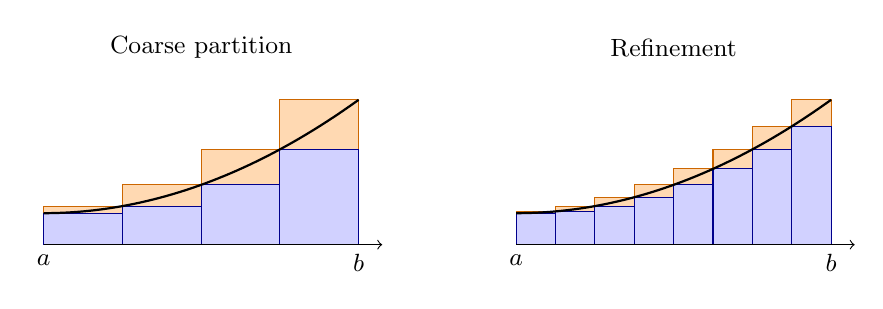
\begin{tikzpicture}[x=1cm,y=1cm,font=\small]
\foreach \shift/\step/\title in {0/1/Coarse partition,6/.5/Refinement}{
\begin{scope}[xshift=\shift cm]
\node at (2,2.5) {\title};
\pgfmathtruncatemacro{\last}{4/\step-1}
\foreach \i in {0,...,\last}{
\pgfmathsetmacro{\a}{\step*\i}
\pgfmathsetmacro{\b}{\a+\step}
\pgfmathsetmacro{\lo}{.4+.09*\a*\a}
\pgfmathsetmacro{\hi}{.4+.09*\b*\b}
\fill[blue!18] (\a,0) rectangle (\b,\lo);
\filldraw[fill=orange!30,draw=orange!80!black] (\a,\lo) rectangle (\b,\hi);
\draw[blue!55!black] (\a,0) rectangle (\b,\lo);
}
\draw[->] (0,0)--(4.3,0);
\draw[thick] plot[domain=0:4,samples=50] (\x,{.4+.09*\x*\x});
\node[below] at (0,0) {$a$};\node[below] at (4,0) {$b$};
\end{scope}}
\end{tikzpicture}
\caption{Blue rectangles give the lower sum; adding the orange bands gives
the upper sum. Inserting cuts raises the lower sum and lowers the upper
sum. The orange area, the Darboux gap, decreases.}
\label{fig:refinement-gap}
\end{figure}

For two partitions use their common refinement
\[
R=P\cup Q.
\]
Then
\[
L(f,P)\leq L(f,R)\leq U(f,R)\leq U(f,Q).
\]
Taking the supremum over $P$ and then the infimum over $Q$ proves
\[
\sup_P L(f,P)\leq\inf_Q U(f,Q).
\]

\begin{proposition}[Darboux criterion]
\label{prop:darboux-criterion}
A bounded function $f:[a,b]\to\R$ is Riemann integrable if and only if, for every $\eps>0$, there is a partition $P$ with
\[
U(f,P)-L(f,P)<\eps.
\]
\end{proposition}
\begin{proof}
Put $L^*=\sup_P L(f,P)$ and $U^*=\inf_P U(f,P)$.  If $f$ is integrable,
then $L^*=U^*=I$.  Given $\eps>0$, choose partitions $P,Q$ such that
\[
U(f,P)<I+\frac{\eps}{2},
\qquad
L(f,Q)>I-\frac{\eps}{2}.
\]
For their common refinement $R$,
\[
L(f,R)\geq L(f,Q)>I-\frac{\eps}{2},
\qquad
U(f,R)\leq U(f,P)<I+\frac{\eps}{2}.
\]
Consequently $U(f,R)-L(f,R)<\eps$.

Conversely, suppose that for every $\eps>0$ there is a partition $P$ with
$U(f,P)-L(f,P)<\eps$.  Then
\[
L(f,P)\leq L^*\leq U^*\leq U(f,P),
\]
and hence
\[
0\leq U^*-L^*\leq U(f,P)-L(f,P)<\eps.
\]
Since this holds for every $\eps>0$, \cref{lem:positive-small} gives
$U^*-L^*=0$.  Thus $L^*=U^*$, so $f$ is Riemann integrable.
\end{proof}

\section{Continuous Functions Are Integrable}

Continuity prevents large oscillation on sufficiently short intervals.
Uniform continuity on a compact interval makes this local control uniform,
which is exactly what the Darboux criterion requires.

\begin{theorem}[Integrability of continuous functions]
\label{thm:continuous-riemann-integrable}
Every continuous function $f:[a,b]\to\R$ is Riemann integrable.
\end{theorem}
\begin{proof}
By \cref{thm:heine-cantor}, $f$ is uniformly continuous, and by the
extreme value theorem it is bounded. Given $\eps>0$, choose $\eta>0$ with
\[
\eta(b-a)<\eps.
\]
Choose $\delta>0$ so that
\[
|x-y|<\delta\quad\Longrightarrow\quad |f(x)-f(y)|<\eta.
\]
Choose, for example, an equal partition $P$ with
$\operatorname{mesh}(P)<\delta$. Then every cell $I_i$ has
$\operatorname{osc}_{I_i}(f)<\eta$. Consequently
\[
U(f,P)-L(f,P)=\sum_i\operatorname{osc}_{I_i}(f)\Delta x_i
<\eta\sum_i\Delta x_i=\eta(b-a)<\eps.
\]
The Darboux criterion proves integrability. Figure~\ref{fig:uniform-bands}
depicts the cellwise height control used in this estimate.
\end{proof}

\begin{figure}[H]
\centering
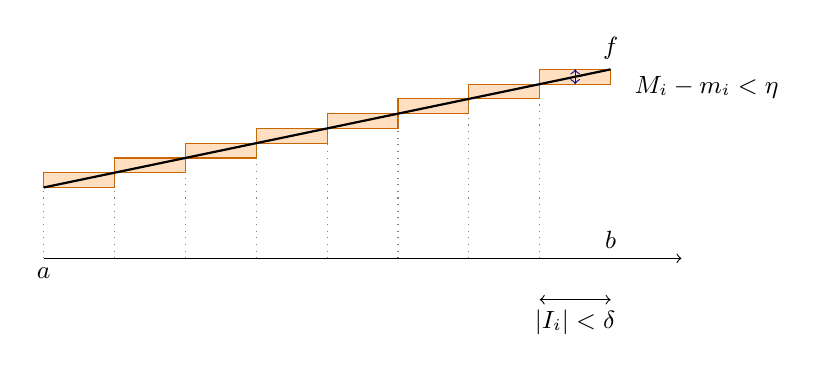
\begin{tikzpicture}[x=1.8cm,y=1.5cm,font=\small]
\foreach \i in {0,...,7}{
\pgfmathsetmacro{\a}{.5*\i}
\pgfmathsetmacro{\b}{\a+.5}
\pgfmathsetmacro{\lo}{.6+.25*\a}
\pgfmathsetmacro{\hi}{.6+.25*\b}
\filldraw[fill=orange!25,draw=orange!80!black] (\a,\lo) rectangle (\b,\hi);
\draw[gray,dotted] (\a,0)--(\a,\lo);
}
\draw[->] (0,0)--(4.5,0);
\draw[thick] (0,.6)--(4,1.6) node[above] {$f$};
\draw[<->,blue!65!black] (3.75,1.475)--(3.75,1.6);
\node[right] at (4.1,1.45) {$M_i-m_i<\eta$};
\draw[<->] (3.5,-.35)--(4,-.35) node[midway,below] {$|I_i|<\delta$};
\node[below] at (0,0) {$a$};\node[above] at (4,0) {$b$};
\end{tikzpicture}
\caption{Uniform continuity makes the vertical oscillation bands narrow
on every sufficiently short cell. Their total area is at most the common
height bound times the full interval length. The strict cell bound shown
here holds for continuous functions since extrema are attained; the proof
needs only the weak bound.}
\label{fig:uniform-bands}
\end{figure}


The elementary oscillation inequalities used below are
\[
\begin{aligned}
\operatorname{osc}_I(f+g)&\leq\operatorname{osc}_I(f)+\operatorname{osc}_I(g),\\
\operatorname{osc}_I(cf)&=|c|\operatorname{osc}_I(f),\\
\operatorname{osc}_I(|f|)&\leq\operatorname{osc}_I(f).
\end{aligned}
\]
They follow from the triangle inequality, homogeneity of absolute value,
and the reverse triangle inequality, applied to pairs of values in $I$.

\begin{theorem}[Basic properties of the integral]
\label{thm:integral-properties}
If $f,g:[a,b]\to\R$ are Riemann integrable and $c\in\R$, then $f+g$ and $cf$ are Riemann integrable, and
\[
\int_a^b(f+g)\,\dd x=\int_a^b f\,\dd x+\int_a^b g\,\dd x,
\qquad
\int_a^b cf\,\dd x=c\int_a^b f\,\dd x.
\]
Moreover, $f\leq g$ implies that their integrals have the same order.
\end{theorem}
\begin{proof}
\textbf{Strategy.} Use one common partition to squeeze both candidate
integral values into the same short interval.

Fix $\eps>0$. By the Darboux criterion, choose partitions $P_f$ and $P_g$ such that
\[
U(f,P_f)-L(f,P_f)<\frac{\eps}{2},
\qquad
U(g,P_g)-L(g,P_g)<\frac{\eps}{2}.
\]
Let $P$ be their common refinement. The oscillation inequality gives
\[
\begin{aligned}
U(f+g,P)-L(f+g,P)
&=\sum_i\operatorname{osc}_{I_i}(f+g)|I_i|\\
&\leq[U(f,P)-L(f,P)]+[U(g,P)-L(g,P)]<\eps.
\end{aligned}
\]
Thus $f+g$ is integrable. Cellwise infimum and supremum inequalities give
\[
L(f,P)+L(g,P)\leq L(f+g,P)
\leq\int_a^b(f+g)\,\dd x
\leq U(f+g,P)\leq U(f,P)+U(g,P),
\]
while separately
\[
L(f,P)+L(g,P)\leq
\int_a^b f\,\dd x+\int_a^b g\,\dd x
\leq U(f,P)+U(g,P).
\]
The common enclosing interval has length
$[U(f,P)-L(f,P)]+[U(g,P)-L(g,P)]<\eps$.
Since $\eps$ is arbitrary, the two values agree.

The scalar oscillation identity proves integrability of $cf$ by the Darboux
criterion (with a sufficiently small gap for $f$ when $c\ne0$).
To identify its integral, for $c>0$ and every interval $I$,
\[
\sup_I(cf)=c\sup_I f,
\qquad
\inf_I(cf)=c\inf_I f.
\]
Thus $U(cf,P)=cU(f,P)$ and $L(cf,P)=cL(f,P)$, which prove both
integrability and the scalar formula by the Darboux criterion.  If $c<0$,
multiplication reverses order, so
\[
\sup_I(cf)=c\inf_I f,
\qquad
\inf_I(cf)=c\sup_I f.
\]
Hence $U(cf,P)=cL(f,P)$ and $L(cf,P)=cU(f,P)$, and the same conclusion
follows; the case $c=0$ is immediate. Finally, if $f\leq g$, then on every
partition interval $I$,
\[
\sup_I f\leq\sup_I g.
\]
Therefore $U(f,P)\leq U(g,P)$ for every partition $P$. Taking infima and
using integrability gives
\[
\int_a^b f\,\dd x\leq\int_a^b g\,\dd x.
\]
\end{proof}

\begin{theorem}[Additivity and absolute-value estimates]
\label{thm:integral-additivity-absolute}
Let $a<c<b$.
\begin{enumerate}
\item If $f:[a,b]\to\R$ is Riemann integrable, then its restrictions to $[a,c]$ and $[c,b]$ are Riemann integrable and
\[
\int_a^b f(x)\,\dd x
=\int_a^c f(x)\,\dd x+\int_c^b f(x)\,\dd x.
\]
\item If $f:[a,b]\to\R$ is Riemann integrable, then $\abs f$ is Riemann integrable and
\[
\left\lvert\int_a^b f(x)\,\dd x\right\rvert
\leq\int_a^b\abs{f(x)}\,\dd x.
\]
\item If $f$ is Riemann integrable and
\[
\abs{f(x)}\leq M
\qquad(x\in[a,b]),
\]
then
\[
\left\lvert\int_a^b f(x)\,\dd x\right\rvert\leq M(b-a).
\]
\end{enumerate}
\end{theorem}
\begin{proof}
For (a), let $\eps>0$ and choose a partition $P$ of $[a,b]$ with
$U(f,P)-L(f,P)<\eps$.  Refine $P$ by inserting $c$; the Darboux gap cannot
increase under refinement.  Let $P_{\mathrm{left}}$ and
$P_{\mathrm{right}}$ be the induced partitions of $[a,c]$ and $[c,b]$.
The sums split as
\[
U_{[a,b]}(f,P)=U_{[a,c]}(f,P_{\mathrm{left}})+U_{[c,b]}(f,P_{\mathrm{right}})
\]
and
\[
L_{[a,b]}(f,P)=L_{[a,c]}(f,P_{\mathrm{left}})+L_{[c,b]}(f,P_{\mathrm{right}}).
\]
Consequently,
\[
U_{[a,b]}-L_{[a,b]}
=(U_{[a,c]}-L_{[a,c]})+(U_{[c,b]}-L_{[c,b]}).
\]
Both terms on the right are nonnegative, so each is less than $\eps$.
The Darboux criterion proves that both restrictions are integrable.

Write
\[
I=\int_a^b f,\qquad I_{\mathrm{left}}=\int_a^c f,\qquad
I_{\mathrm{right}}=\int_c^b f.
\]
For every partition containing $c$, the
split lower and upper sums give
\[
L_{[a,b]}(f,P)\leq I_{\mathrm{left}}+I_{\mathrm{right}}
\leq U_{[a,b]}(f,P).
\]
Choose such a partition with $U_{[a,b]}(f,P)-L_{[a,b]}(f,P)<\eps$.  Since
$L_{[a,b]}(f,P)\leq I\leq U_{[a,b]}(f,P)$, it follows that
\[
I-\eps<I_{\mathrm{left}}+I_{\mathrm{right}}<I+\eps.
\]
As this holds for every $\eps>0$, the desired additivity identity follows.

For (b), the inequality
\[
\bigl\lvert\abs{u}-\abs{v}\bigr\rvert\leq\abs{u-v}
\]
implies that, for $x,y$ in a partition interval $I_i$,
\[
\bigl\lvert\abs{f(x)}-\abs{f(y)}\bigr\rvert\leq\abs{f(x)-f(y)}.
\]
Thus
\[
\operatorname{osc}_{I_i}(|f|)\leq\operatorname{osc}_{I_i}(f),
\qquad U(|f|,P)-L(|f|,P)\leq U(f,P)-L(f,P).
\]
The Darboux criterion proves integrability of $\abs f$. Since
\[
-\abs f\leq f\leq\abs f,
\]
\cref{thm:integral-properties} gives
\[
-\int_a^b\abs f\,\dd x\leq\int_a^b f\,\dd x
\leq\int_a^b\abs f\,\dd x,
\]
which yields the stated inequality.  For (c), order preservation applied to
\[
0\leq\abs f\leq M.
\]
gives
\[
\int_a^b\abs f\,\dd x\leq\int_a^b M\,\dd x=M(b-a).
\]
Combine this with (b).
\end{proof}

\begin{theorem}[Integral H\"older and Cauchy--Schwarz inequalities]
\label{thm:integral-holder}
Let \(p,q>1\) be conjugate exponents, and let \(f,g\) be continuous on
\([a,b]\). Then
\[
\boxed{
\int_a^b|f(x)g(x)|\,\dd x
\leq
\left(\int_a^b|f(x)|^p\,\dd x\right)^{1/p}
\left(\int_a^b|g(x)|^q\,\dd x\right)^{1/q}.}
\]
\end{theorem}
\begin{proof}
Set
\[
A=\left(\int_a^b|f|^p\right)^{1/p},
\qquad
B=\left(\int_a^b|g|^q\right)^{1/q}.
\]
If \(A=0\), continuity and nonnegativity imply \(f=0\) throughout the
interval: a nonzero value would persist on a short interval and force a
positive integral. The same applies when \(B=0\). Otherwise Young's inequality
\cref{cor:young-inequality}, applied pointwise to \(|f|/A\) and \(|g|/B\),
gives
\[
\frac{|fg|}{AB}
\leq\frac{|f|^p}{pA^p}+\frac{|g|^q}{qB^q}.
\]
Integrate and use \(1/p+1/q=1\), then multiply by \(AB\).
\end{proof}

For \(p=q=2\), the absolute-value estimate for integrals gives the
\textbf{integral Cauchy--Schwarz inequality}
\[
\boxed{
\left|\int_a^b f(x)g(x)\,\dd x\right|
\leq
\left(\int_a^b|f(x)|^2\,\dd x\right)^{1/2}
\left(\int_a^b|g(x)|^2\,\dd x\right)^{1/2}.}
\]
Taking \(g\equiv1\) in H\"older also gives
\[
\int_a^b|f(x)|\,\dd x
\leq(b-a)^{1/q}
\left(\int_a^b|f(x)|^p\,\dd x\right)^{1/p}.
\]
These are Riemann-integral consequences of Young's inequality; no
\(L^p\) theory is being introduced. Chapter~\ref{ch:topology-linear-algebra}
later interprets the \(p=2\) case through an integral inner product.

\begin{theorem}[Integrability of monotone functions]
\label{thm:monotone-riemann-integrable}
Every monotone function $f:[a,b]\to\R$ is Riemann integrable.
\end{theorem}
\begin{proof}
It is enough to consider an increasing function; the decreasing case follows by applying the result to $-f$. For a partition $P$, monotonicity gives
\[
M_i=f(x_i),
\qquad
m_i=f(x_{i-1}).
\]
Thus
\[
U(f,P)-L(f,P)
=\sum_{i=1}^{n}\bigl(f(x_i)-f(x_{i-1})\bigr)(x_i-x_{i-1})
\leq\operatorname{mesh}(P)\sum_{i=1}^{n}\bigl(f(x_i)-f(x_{i-1})\bigr).
\]
Here $x_i-x_{i-1}\leq\operatorname{mesh}(P)$ and each difference
$f(x_i)-f(x_{i-1})$ is nonnegative.  The sum telescopes:
\[
\sum_{i=1}^{n}\bigl(f(x_i)-f(x_{i-1})\bigr)=f(b)-f(a).
\]
Therefore
\[
U(f,P)-L(f,P)\leq\operatorname{mesh}(P)\bigl(f(b)-f(a)\bigr).
\]
Choose a partition with norm less than
\[
\frac{\eps}{f(b)-f(a)}
\]
when $f(b)>f(a)$; if $f(b)=f(a)$, the function is constant and the upper and lower sums are equal. The Darboux criterion proves integrability.
\end{proof}

\subsection{Tagged sums: the calculus meaning of the integral}

Darboux sums enclose an accumulated quantity without sampling the function.
Calculus computations usually sample once in each cell instead. We must
show that every sufficiently fine sampling gives the same answer, regardless
of the tags and without requiring nested partitions.

Fix a coarse partition first. A fine cell lying inside one old cell
inherits its oscillation bound. A \emph{crossing cell} has an old interior
division point in its interior; it needs only the global height bound.
Each old point lies in the interior of at most one fine cell. Thus there
are at most as many crossing cells as old interior division points.
Figure~\ref{fig:fine-crossing} displays these two contributions.
\begin{figure}[H]
\centering
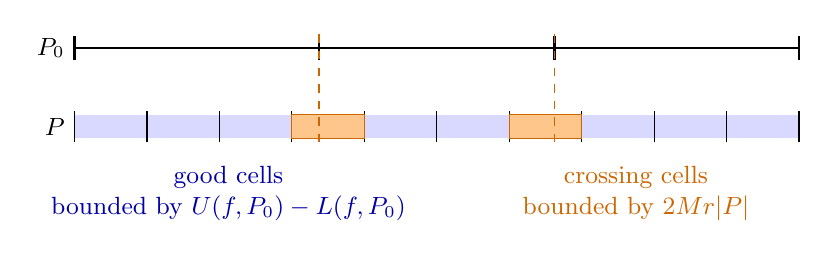
\begin{tikzpicture}[x=1.15cm,y=1cm,font=\small]
\node[left] at (0,1) {$P_0$};
\node[left] at (0,0) {$P$};
\draw[thick] (0,1)--(8,1);
\foreach \x in {0,2.7,5.3,8}{\draw[thick] (\x,.85)--(\x,1.15);}
\foreach \i in {0,...,9}{
\pgfmathsetmacro{\a}{.8*\i}
\pgfmathsetmacro{\b}{\a+.8}
\filldraw[fill=blue!15,draw=white] (\a,-.15) rectangle (\b,.15);
\draw (\a,-.2)--(\a,.2);
}
\foreach \a/\b in {2.4/3.2,4.8/5.6}{
\filldraw[fill=orange!45,draw=orange!80!black] (\a,-.15) rectangle (\b,.15);}
\draw (8,-.2)--(8,.2);
\foreach \x in {2.7,5.3}{\draw[dashed,orange!80!black] (\x,-.2)--(\x,1.25);}
\node[blue!65!black,align=center] at (1.7,-.85) {good cells\\bounded by $U(f,P_0)-L(f,P_0)$};
\node[orange!80!black,align=center] at (6.2,-.85) {crossing cells\\bounded by $2Mr|P|$};
\end{tikzpicture}
\caption{A fine partition need not refine the coarse one. Blue cells inherit
the coarse oscillation bounds; orange cells cross old division points.
Their total width is at most $r|P|$, so their gap contribution is at most
$2Mr|P|$.}
\label{fig:fine-crossing}
\end{figure}


For a partition $P:a=x_0<\cdots<x_m=b$, choose tags
$\xi_i\in[x_{i-1},x_i]$. Its tagged sum is

\[
S(f,P,\xi)=\sum_i f(\xi_i)(x_i-x_{i-1});
\]
 its mesh is
$\operatorname{mesh}(P)=\max_i(x_i-x_{i-1})$.

\begin{theorem}[Fine-mesh characterization]
\label{thm:tagged-riemann}
A bounded function $f:[a,b]\to\R$ is Riemann integrable with integral $I$
if and only if for every $\eps>0$ there is $\delta>0$ such that every tagged
partition of mesh less than $\delta$ satisfies $|S(f,P,\xi)-I|<\eps$.
\end{theorem}
\begin{proof}
Suppose $f$ is integrable and $|f|\leq M$. Choose a coarse partition
$P_0$ such that
\[
U(f,P_0)-L(f,P_0)<\frac\eps2,
\]
and let $r$ be its number of interior division points. For any partition
$P$, the good cells inside a fixed coarse cell have total length at most
that coarse cell's length, and their oscillations are no larger. More
explicitly, if $I_j$ is a coarse cell and $\mathcal G_j$ is the family of
fine cells contained in it, then
\[
\sum_{J\in\mathcal G_j}\operatorname{osc}_J(f)\ell(J)
\leq\operatorname{osc}_{I_j}(f)
\sum_{J\in\mathcal G_j}\ell(J)
\leq\operatorname{osc}_{I_j}(f)\ell(I_j).
\]
Summing over $j$ bounds all good cells by the coarse Darboux gap. There are
at most $r$ crossing cells, each of length at most $\operatorname{mesh}(P)$ and oscillation
at most $2M$. Therefore
\[
U(f,P)-L(f,P)<\frac\eps2+2Mr\operatorname{mesh}(P).
\]
If $Mr>0$, choose $\delta>0$ so small that
\[
2Mr\delta<\frac\eps2.
\]
If $Mr=0$, the crossing contribution is already zero and any $\delta>0$
works. On each fine cell, $m_i\leq f(\xi_i)\leq M_i$; multiplying by
$\Delta x_i$ and summing gives
\[
L(f,P)\leq S(f,P,\xi)\leq U(f,P).
\]
For $\operatorname{mesh}(P)<\delta$, both $I$ and every tagged sum therefore
lie between $L(f,P)$ and $U(f,P)$, whose gap is less than $\eps$.

Conversely, fix $\eps>0$, use the tagged-sum hypothesis with tolerance
\[
\frac\eps4,
\]
and choose a partition $P$ with sufficiently small mesh. Choose $\eta>0$
once so that
\[
\eta(b-a)<\frac\eps4.
\]
On each cell choose near-supremum and near-infimum tags satisfying
\[
f(\xi_i)>M_i-\eta,\qquad f(\zeta_i)<m_i+\eta.
\]
No attained extrema are required. Summing gives
\[
\begin{aligned}
0\leq U(f,P)-S(f,P,\xi)&<\eta(b-a)<\frac\eps4,\\
0\leq S(f,P,\zeta)-L(f,P)&<\eta(b-a)<\frac\eps4.
\end{aligned}
\]
Both tagged sums are within the chosen tolerance of $I$, so
\[
U(f,P)<I+\frac\eps2,\qquad L(f,P)>I-\frac\eps2.
\]
The gap is less than $\eps$, proving integrability by the Darboux
criterion. Its integral $J$ lies between the same sums; hence
\[
|J-I|<\frac\eps2.
\]
Since $\eps>0$ was arbitrary, $J=I$.
\end{proof}
Thus sampled values times interval widths approximate the integral, with
an error controlled by the mesh independently of the sample choices.

\subsection*{Deciding integrability in ordinary problems}
For a function on \([a,b]\), the available tests depend on its regularity.
\begin{enumerate}[label=\arabic*.,leftmargin=*]
\item Check boundedness. Without it, the proper Riemann integral is not
defined.
\item Check continuity on the whole compact interval; if it holds,
\cref{thm:continuous-riemann-integrable} settles the question.
\item If continuity fails, check monotonicity.
\item Check whether the function is bounded and piecewise continuous with
only finitely many jumps.
\item If no theorem applies immediately, construct a partition for which
\(U(f,P)-L(f,P)\) is small.
\item To disprove integrability, look instead for a fixed positive lower
bound on \(U(f,P)-L(f,P)\) that survives every partition.
\item After \cref{thm:riemann-lebesgue-criterion} is available, use the
Lebesgue criterion when the discontinuity set is easier to analyze than
partitions are.
\end{enumerate}
Continuity and monotonicity supply the first two positive tests just proved.

\begin{theorem}[Finitely many discontinuities]
\label{thm:finite-discontinuities-integrable}
A bounded function on $[a,b]$ that is continuous except at finitely many
points is Riemann integrable. In particular, every piecewise-continuous
function in the sense of \cref{def:piecewise-continuous} is integrable.
\end{theorem}
\begin{proof}
The mechanism is
\[
\boxed{\text{one bad point}\longrightarrow\text{one short bad interval}
\longrightarrow\text{finitely many bad points}.}
\]
Suppose first that only $c$ is exceptional and choose $M$ with
$|f|\leq M$. Enclose $c$ in an interval of length less than
$\eps/[4(M+1)]$. On the two remaining closed pieces, continuity and
\cref{thm:continuous-riemann-integrable} give partitions whose combined
Darboux gap is less than $\eps/2$. Insert the endpoints of the short bad
interval. Its oscillation is at most $2M$, so its contribution is less
than $\eps/2$.

For finitely many exceptional points, choose their surrounding intervals
with total length
\[
\ell<\frac{\eps}{4(M+1)}.
\]
Repeat the preceding construction on the finitely many complementary
closed pieces. With $\mathcal G$ and $\mathcal E$ denoting the good and bad
cells of the resulting common partition,
\[
\begin{aligned}
U(f,P)-L(f,P)
&=\sum_{I\in\mathcal G}\operatorname{osc}_I(f)\ell(I)
 +\sum_{I\in\mathcal E}\operatorname{osc}_I(f)\ell(I),\\
\sum_{I\in\mathcal E}\operatorname{osc}_I(f)\ell(I)
&\leq2M\sum_{I\in\mathcal E}\ell(I)\leq2M\ell<\eps/2.
\end{aligned}
\]
The good contribution was chosen below $\eps/2$, so the Darboux criterion
proves the result.
\end{proof}

\begin{example}[A direct Darboux calculation]
For $f(x)=x^2$ on $[0,1]$, the equal partition $P_n$ has
\[
U(f,P_n)-L(f,P_n)
=\frac1n\sum_{k=1}^n
\left(\left(\frac kn\right)^2-\left(\frac{k-1}{n}\right)^2\right)
=\frac1n.
\]
Given $\eps>0$, choose
\[
n>1/\eps;
\]
 the Darboux criterion proves
integrability directly. For the step function that is zero on

\[
[0,1/2)
\]
 and one on
\[
[1/2,1],
\]
 isolate the jump in

\[
[1/2-\eta,1/2+\eta],
\]
 where
\[
0<\eta<\min\{1/2,\eps/2\}.
\]

Every other cell has zero oscillation; the gap is at most $2\eta<\eps$.
\end{example}

To prove nonintegrability it suffices to find $c>0$ such that
$U(f,P)-L(f,P)\geq c$ for \emph{every} partition $P$.
For $\mathbf1_{\Q}$ on $[0,1]$, rational and irrational density make
every cell's supremum $1$ and infimum $0$. Thus the gap is always $1$.
The later \cref{ex:dirichlet-function,ex:thomae-function} contrast a fixed
gap on every interval with a function whose large oscillations can be
confined to intervals of arbitrarily small total length. Together with the
continuous, monotone, and finite-jump cases above, they show why choosing an
efficient integrability test is part of the problem.

\section{Uniform Limits and Integration}

An integral is itself a limit, so a second limiting process must be handled
with care.  In the Riemann theory, uniform convergence is the clean
condition that permits a limit to pass through an integral: one error bound
works on the whole interval and hence controls the accumulated error.

\Needspace{20\baselineskip}
\begin{theorem}[Uniform interchange of limits and Riemann integrals]
\label{thm:uniform-riemann-integration}
Let
\[
f_n:[a,b]\longrightarrow\R
\]
be Riemann integrable for every \(n\), and suppose that \(f_n\) converges
uniformly on \([a,b]\) to a function \(f\).  Then \(f\) is Riemann
integrable and
\[
\lim_{n\to\infty}\int_a^b f_n(x)\,\dd x
=
\int_a^b f(x)\,\dd x.
\]
In fact,
\[
\lim_{n\to\infty}\int_a^b\abs{f_n(x)-f(x)}\,\dd x=0.
\]
\end{theorem}
\begin{proof}
\textbf{Stage 1: integrability of the limit.}
Put $d_n=\|f-f_n\|_\infty$. For $x,y$ in any interval $I$,
\[
|f(x)-f(y)|\leq|f(x)-f_n(x)|+|f_n(x)-f_n(y)|
                   +|f_n(y)-f(y)|,
\]
so
\[
\operatorname{osc}_I(f)\leq\operatorname{osc}_I(f_n)+2d_n.
\]
Consequently, for every partition $P$,
\[
U(f,P)-L(f,P)
\leq U(f_n,P)-L(f_n,P)+2d_n(b-a).
\]
Given $\eps>0$, first choose $n$ so that $2d_n(b-a)<\eps/2$, and then
choose $P$ so that the Darboux gap of $f_n$ is below $\eps/2$. The Darboux
criterion proves that $f$ is integrable.

\textbf{Stage 2: convergence of the integrals.}
The basic integral estimates give the sup-norm bound
\[
\left\lvert
\int_a^b f_n\,\dd x-\int_a^b f\,\dd x
\right\rvert
\leq
\int_a^b\abs{f_n-f}\,\dd x
\leq
(b-a)\sup_{x\in[a,b]}\abs{f_n(x)-f(x)}.
\]
The right-hand side tends to zero.  The same final estimate proves the last
assertion.
\end{proof}

\paragraph{Corollary: integrating a uniformly convergent series.}
If
\[
\sum_{n=1}^{\infty}f_n
\]
converges uniformly on $[a,b]$ and each $f_n$
is Riemann integrable, then its sum is Riemann integrable and
\[
\int_a^b\left(\sum_{n=1}^{\infty}f_n(x)\right)\,\dd x
=\sum_{n=1}^{\infty}\int_a^b f_n(x)\,\dd x.
\]
Apply \cref{thm:uniform-riemann-integration} to the partial sums and use
linearity for each finite sum.

\subsection{Pointwise bounded convergence requires a different argument}
\label{thm:dominated-uniform-riemann}
Uniform convergence provides a single bound on all pointwise errors.
Pointwise convergence does not: a bad location may move with $n$.
Nevertheless bounded heights and an integrable limit suffice for integral
convergence. We need an elementary fact about intervals.
We prove it explicitly, without introducing Lebesgue integration.

The open-cover, relative-topology, compactness, finite-subcover, and
common-scale terminology used below is established in
\cref{sec:real-line-topology,sec:real-line-compactness}.

For an open subset $G$ of $(a,b)$, use the component-interval decomposition
of \cref{prop:real-open-interval-components} and define
\[
\ell(G)=\sum_j\ell(I_j),\qquad \ell((u,v))=v-u,
\]
where $G=\bigsqcup_j I_j$.
Every finite sum of their lengths is at most $b-a$, so the full sum
exists. This definition is only a tool for open interval covers.
\begin{lemma}[Two elementary facts about open-set lengths]
\label{lem:open-length-tool}
If an open $G$ is contained in
\[
\bigcup_jG_j
\]
 with the $G_j$ open,
then
\[
\ell(G)\leq\sum_j\ell(G_j).
\]
 Also, for every $\eta>0$ an
open $G\subset(a,b)$ contains a finite union $K$ of compact intervals
such that $\ell(G\setminus K)<\eta$.
\end{lemma}
\begin{proof}
\textbf{Claim 1: inner approximation.} If $\ell(K)$ denotes the combined
length of a finite union of disjoint closed intervals, then
\[
\ell(G)=\sup\{\ell(K):K\subset G,\ K\text{ a finite union of closed intervals}\}.
\]
Indeed, retain finitely many component intervals of $G$ and shorten their
endpoints slightly. These finite inner approximations approach the defining
component sum from below.

\textbf{Claim 2: finite interval covers.} If finitely many open intervals
cover a finite union $K$ of disjoint closed intervals, their total length
is at least $\ell(K)$. Sort all endpoints and subdivide at them. Every
subinterval belonging to $K$ is counted at least once among the covering
lengths, which proves the inequality.

\textbf{Claim 3: reduce to the finite case.} The component intervals of
all $G_j$ form an open cover of any such $K$. Compactness from
\cref{cor:closed-subset-finite-subcover} selects a finite subcover, and
Claim~2 gives
\[
\ell(K)\leq\sum_j\ell(G_j).
\]
Taking the supremum over $K$ in Claim~1 proves subadditivity.

\textbf{Claim 4: finite approximation with controlled loss.} Retain
finitely many components of $G$ whose omitted tail has length less than
\[
\eta/2;
\]
then shorten those retained intervals by a combined length less than
\[
\eta/2.
\]
Their compact union is $K$, and the components of $G\setminus K$ consist of the
discarded tail and endpoint strips. Their total length is less than $\eta$.
\end{proof}
\begin{lemma}[Nested open sets of uniformly positive length]
\label{lem:nested-open-length}
If $G_n\subset(a,b)$ are decreasing open sets and
$\ell(G_n)\geq c>0$ for every $n$, then
\[
\bigcap_nG_n\ne\varnothing.
\]

\end{lemma}
\begin{proof}
The roadmap is
\[
G_n\supset K_n\longrightarrow H_m=K_1\cap\cdots\cap K_m
\longrightarrow H_m\ne\varnothing
\longrightarrow\bigcap_mH_m\ne\varnothing.
\]
The sets \(G_n\) are open, so the nested-closed-set argument does not apply
directly. Choose finite unions of closed bounded intervals
$K_n\subset G_n$ with
\[
\ell(G_n\setminus K_n)<c/2^{n+1}.
\]

The approximations $K_n$ need not be nested: shortening and retaining
different intervals at each stage makes independent choices. Set

\[
H_m=K_1\cap\cdots\cap K_m
\]
 instead. It is a finite union of closed bounded intervals (possibly
degenerate), hence satisfies the local finite-subcover result just proved,
and $H_{m+1}\subseteq H_m$. We must still show
nonemptiness; the summable errors were chosen for exactly this purpose.
If $H_m$ were empty, then every $x\in G_m$ belongs to $G_i$ for $i\leq m$
by nestedness, but failure of membership in $H_m$ means that $x\notin K_i$
for at least one such $i$. Hence
\[
G_m\subset\bigcup_{i=1}^m(G_i\setminus K_i),\qquad
\ell(G_m)<\sum_{i=1}^m c/2^{i+1}<c/2,
\]
contradicting its lower bound. The nonempty sets \(H_m\), each a finite
union of closed bounded intervals, decrease inside \([a,b]\), so their
intersection is nonempty. Explicitly, otherwise
the open complements of the $H_m$ would finitely cover $H_1$, forcing
one late $H_m$ to be empty. A point in every $H_m$ belongs to every $G_n$.
\end{proof}
\begin{theorem}[Arzel\`a bounded convergence]
\label{thm:arzela-bounded-riemann}
Let $f_n:[a,b]\to\R$ be Riemann integrable, $f_n\to f$ pointwise,
and $|f_n(x)|\leq M$ for all $n,x$. If $f$ is Riemann integrable,
then
\[
\int_a^b|f_n-f|\longrightarrow0,\qquad
\int_a^b f_n\longrightarrow\int_a^b f.
\]
\end{theorem}
\begin{proof}
The proof follows
\[
\boxed{\text{large error integral}\Rightarrow\text{large bad set}
\Rightarrow\text{one fixed point is bad infinitely often}
\Rightarrow\text{contradiction}.}
\]
Let $g_n=|f_n-f|$. These are integrable by the integral algebra already
proved, satisfy $0\leq g_n\leq2M$, and tend pointwise to zero.
The cases $a=b$ or $M=0$ are immediate. If the integrals do not tend to
zero, pass to a subsequence and choose $\eta>0$ such that
\[
\int_a^b g_n\geq\eta
\]
for every term of the subsequence. Put
\[
h=\frac{\eta}{2(b-a)}.
\]
For each $n$, integrability supplies a lower Darboux sum greater than
$3\eta/4$. Call a cell low when its lower height is at most $h$ and high
otherwise. The low cells contribute at most $h(b-a)=\eta/2$, so the high
cells contribute more than $\eta/4$. Because all heights are at most
$2M$, their combined length is at least
\[
c=\frac{\eta}{8M}>0.
\]
Let $U_n$ be the union of the interiors of the high cells. Endpoints do not
change interval length, so $\ell(U_n)\geq c$, and $g_n>h$ on $U_n$.
The open sets
\[
G_N=\bigcup_{n\geq N}U_n
\]
decrease and each has length at least $c$. By
\cref{lem:nested-open-length}, some
$x$ belongs to every $G_N$. Unpacking the union and intersection,
\[
x\in\bigcap_NG_N\quad\Longleftrightarrow\quad
\text{for every }N\text{ there exists }n\geq N\text{ with }x\in U_n.
\]
It is one fixed point $x$ lying in arbitrarily late bad sets, so
$g_n(x)>h$ at arbitrarily large indices. Pointwise convergence at this
fixed $x$ says all sufficiently late errors are less than $h$, a
contradiction. The point cannot vary with $N$ in this last step. This proves convergence of the absolute
error integrals. Finally

\[
|\int f_n-\int f|\leq\int|f_n-f|
\]
 proves the second assertion.
\end{proof}
\begin{example}[The limit's integrability cannot be dropped]
Enumerate the rationals in $[0,1]$ as $q_1,q_2,\ldots$ and set
$f_n=\mathbf1_{\{q_1,\ldots,q_n\}}$. A finite set is covered by
finitely many intervals of arbitrarily small total length, so each
$f_n$ has integral zero. Also $0\leq f_n\leq1$ and $f_n$ converges
pointwise to $\mathbf1_\Q$. Every nondegenerate interval contains both
rational and irrational points, so the limit has lower sum $0$ and upper
sum $1$ for every partition. It is not Riemann integrable.
\end{example}
Uniform Riemann interchange automatically supplies an integrable limit.
Arzel\`a's theorem permits pointwise convergence but separately assumes
that integrability. Neither theorem permits arbitrary unbounded moving
spikes. Bartle~\cite{bartle-elements} is a classical companion for comparing
these convergence hypotheses; the interval-cover proof above is internal.

Measure-theoretic convergence theorems weaken these hypotheses
substantially; they are stated and compared with the present Riemann results
in Section~9.7. Dini's theorem itself now appears in
Chapter~\ref{ch:function-sequences}.

\section{The Fundamental Theorem of Calculus}

Differentiation measures local change, while integration accumulates local
change.  The Fundamental Theorem identifies these two operations under the
continuity hypotheses that make both constructions stable. In the familiar
elementary setting one often has \(F\in C^1\), in the one-variable sense of
\cref{def:one-variable-ck}, so \(F'\) is continuous. The results below first
work in that comfortable setting and then identify exactly which hypotheses
can be weakened.

\begin{proposition}[Accumulation at continuity points]
\label{prop:ftc-continuity-points}
For Riemann-integrable $f$ on $[a,b]$, the accumulation function
\[
F(x)=\int_a^x f(t)\,\dd t
\]
is continuous. Here $x$ is the free
endpoint parameter and $t$ is a bound integration variable. Renaming $t$
does not change the function $F$.
At every interior point $c$ where $f$ is continuous, $F'(c)=f(c)$.
\end{proposition}
\begin{proof}
If $|f|\leq M$, additivity and the integral bound give
$|F(y)-F(x)|\leq M|y-x|$, so $F$ is continuous.
For $h>0$ with $c+h\in[a,b]$, additivity first gives the increment identity
\[
\frac{F(c+h)-F(c)}h-f(c)=\frac1h\int_c^{c+h}(f(t)-f(c))\,\dd t.
\]
For $h<0$ use only forward-endpoint integrals at this stage:
\[
\frac{F(c+h)-F(c)}h-f(c)
=\frac1{-h}\int_{c+h}^{c}(f(t)-f(c))\,\dd t.
\]
In either case the absolute error is at most
$\sup\{|f(t)-f(c)|:|t-c|\leq|h|,\ t\in[a,b]\}$.
Given $\eps>0$, continuity at $c$ supplies a neighborhood on which

\[
|f(t)-f(c)|<\eps/2.
\]
 Choose $|h|$ small enough that the whole interval
of integration lies there. The supremum is at most
\[
\eps/2<\eps,
\]

so the difference quotient tends to $f(c)$.
\end{proof}

\begin{corollary}[Fundamental theorem of calculus, first part]
\label{thm:ftc-one}
Let $f:[a,b]\to\R$ be continuous and define
\[
F(x)=\int_a^x f(t)\,\dd t.
\]
Then $F$ is differentiable on $(a,b)$ and $F'(x)=f(x)$.
\end{corollary}
\begin{proof}
Continuity makes $f$ Riemann integrable and makes every interior point a
continuity point. Apply \cref{prop:ftc-continuity-points} at each such point.
\end{proof}

\begin{theorem}[Fundamental theorem of calculus, second part]
\label{thm:ftc-two}
Let $F:[a,b]\to\R$ be differentiable on $(a,b)$ and continuous on $[a,b]$. Suppose that its derivative extends to a continuous function $f:[a,b]\to\R$, so that
\[
F'(x)=f(x)
\qquad\text{for every }x\in(a,b).
\]
Then
\[
\int_a^b f(x)\,\dd x=F(b)-F(a).
\]
\end{theorem}
\begin{proof}
Define
\[
G(x)=\int_a^x f(t)\,\dd t.
\]
By \cref{thm:ftc-one}, $G'(x)=f(x)$ for $x\in(a,b)$. Therefore the function $H=F-G$ is continuous on $[a,b]$, differentiable on $(a,b)$, and satisfies $H'(x)=0$ throughout $(a,b)$. For $x=a$, the identity
\[
H(x)=H(a)
\]
is immediate. If $x\in(a,b]$, the Mean Value Theorem applied on $[a,x]$ gives a point $c\in(a,x)$ for which
\[
H(x)-H(a)=H'(c)(x-a)=0.
\]
Thus $H$ is constant. Since $G(a)=0$, evaluating at $b$ gives
\[
F(b)-F(a)=G(b)=\int_a^b f(x)\,\dd x.
\]
\end{proof}

\subsection{Antiderivatives and indefinite integrals}

\begin{definition}[Antiderivative]
\label{def:antiderivative}
Let \(f:I\to\R\) be defined on an interval \(I\). A differentiable function
\(F:I\to\R\) is an \textbf{antiderivative} of \(f\) on \(I\) if
\[
F'(x)=f(x)
\qquad(x\in I),
\]
with one-sided derivatives at included endpoints when appropriate.
\end{definition}

\begin{proposition}[Antiderivatives differ by a constant]
\label{prop:antiderivatives-constant}
If \(F\) and \(G\) are antiderivatives of the same function on an interval
\(I\), then there is a constant \(C\) such that
\[
F(x)-G(x)=C
\qquad(x\in I).
\]
\end{proposition}
\begin{proof}
Put \(H=F-G\). Then \(H'=0\) on the interior of \(I\). For any \(x<y\)
in \(I\), the Mean Value Theorem on \([x,y]\) gives a point \(c\in(x,y)\)
such that
\[
H(y)-H(x)=H'(c)(y-x)=0.
\]
Thus \(H\) has one value throughout \(I\).
\end{proof}

This proposition is the rigorous reason for the arbitrary constant in
\[
\int f(x)\,\dd x=F(x)+C.
\]
The expression on the left is \textbf{indefinite-integral notation}: it
denotes the family of all antiderivatives on the interval under discussion.
It is not a definite Riemann integral with its endpoints deleted. The
distinction is one of type:
\[
\begin{array}{c|c}
\text{definite integral }\displaystyle\int_a^b f(x)\,\dd x
&\text{a number}\cr
\text{indefinite integral }\displaystyle\int f(x)\,\dd x
&\text{a family of functions }F+C.
\end{array}
\]
The interval hypothesis matters. On \(\R\setminus\{0\}\), two
antiderivatives of
\[
1/x
\]
 may differ by one constant on
\((\! -\infty,0)\) and by another on \((0,\infty)\). Thus
\[
\int\frac{\dd x}{x}=\log|x|+C
\]
is understood on one interval avoiding zero. More generally, one constant
is available on each maximal interval contained in the domain.

In the first line below, $F$ is the accumulation function just defined.
The two FTC statements read in opposite directions:
\[
\boxed{
\begin{aligned}
\text{FTC I:}\quad
f\text{ continuous}
&\Longrightarrow
F'(x)=f(x),\quad x\in(a,b),\\
\text{FTC II:}\quad
F'=f
&\Longrightarrow
\int_a^b f(x)\,\dd x=F(b)-F(a)
\quad\text{under the stated continuity hypotheses.}
\end{aligned}}
\]
FTC I says that integrating a continuous rate produces an antiderivative.
FTC II, or the Newton--Leibniz formula, is the direction most often used in
elementary calculations: recognize \(F\), verify \(F'=f\), and evaluate the
endpoints. Also,
\[
\boxed{\text{having an antiderivative}
\ne
\text{having an elementary closed-form antiderivative}.}
\]
For every continuous \(f\), FTC I supplies the perfectly valid
antiderivative
\[
x\mapsto\int_a^x f(t)\,\dd t,
\]
 even when no familiar
elementary formula is available.

\begin{example}[The two directions of the FTC]
The integral
\[
A(x)=\int_0^x(1+t^2)\,\dd t
\]
 for $x>0$ defines an antiderivative:
the first part of the FTC gives $A'(x)=1+x^2$ directly from continuity
of the integrand. Conversely, once
\[
B(x)=x+x^3/3
\]
 is known to satisfy
$B'(x)=1+x^2$, the second part evaluates
\[
\int_0^2(1+x^2)\,\dd x=[x+x^3/3]_0^2=2+8/3=14/3.
\]
The first use constructs an antiderivative from an integral; the second
uses an antiderivative to evaluate a definite integral.
\end{example}

\begin{example}[A basic antiderivative library]
\label{ex:inverse-trigonometric-antiderivatives}
Each entry below is justified by differentiating the proposed
antiderivative and checking its domain:
\[
\begin{array}{c|c}
\text{integrand}&\text{antiderivative}\cr\hline
x^p&\dfrac{x^{p+1}}{p+1}+C\quad(p\ne-1)\cr
1/x&\log|x|+C\cr
e^x&e^x+C\cr
a^x&\dfrac{a^x}{\log a}+C\quad(a>0,\ a\ne1)\cr
\sin x&-\cos x+C\cr
\cos x&\sin x+C\cr
1/\cos^2x&\tan x+C\cr
1/(1+x^2)&\arctan x+C\cr
1/\sqrt{1-x^2}&\arcsin x+C\cr
-1/\sqrt{1-x^2}&\arccos x+C.
\end{array}
\]
For arbitrary real \(p\), the power formula holds on intervals contained in
\((0,\infty)\), where Chapter~\ref{ch:differentiation} defines \(x^p\).
It also holds on any larger real domain on which the relevant power is
defined and the derivative formula is valid. The logarithmic formula is
used only on an interval avoiding zero. The tangent formula requires
\(\cos x\ne0\), and the arcsine formula is used on intervals contained in
\((-1,1)\).

Representative checks reveal the mechanisms behind the table. For real
powers on the positive half-line,
\[
\frac{\dd}{\dd x}\left(\frac{x^{p+1}}{p+1}\right)
=\frac{p+1}{p+1}x^p=x^p\qquad(p\ne-1).
\]
The sine, cosine, exponential, tangent, and arctangent entries follow by
the same reversal of their established derivatives. The arcsine entry uses
\[
\frac{\dd}{\dd x}\arcsin x=\frac1{\sqrt{1-x^2}}\qquad(-1<x<1).
\]
By the principal-range identity from Chapter~8,
\[
\arcsin x+\arccos x=\frac\pi2.
\]
Thus the same antiderivative family can equally be written
\[
\int\frac{\dd x}{\sqrt{1-x^2}}
=\arcsin x+C_1=-\arccos x+C_2\qquad(-1<x<1),
\]
where the arbitrary constants are adjusted by the fixed difference.

\paragraph{Why the logarithm contains an absolute value.}
The real logarithm retains its domain
\[
\log:(0,\infty)\longrightarrow\R.
\]
For $x>0$ its derivative is the reciprocal. For $x<0$, the positive
argument $-x$ is available, and the chain rule gives
\[
\frac{\dd}{\dd x}\log(-x)=\frac1{-x}(-1)=\frac1x.
\]
Since $|x|=x$ on the positive half-line and $|x|=-x$ on the negative
half-line, these two checks prove
\[
\int\frac{\dd x}{x}=\log|x|+C
\]
on each interval avoiding zero. No logarithm of a negative number is used.
For a differentiable $g$ that is nonzero throughout an interval, continuity
and the intermediate value theorem make its sign constant. Applying the
same two cases and the chain rule gives
\[
\frac{\dd}{\dd x}\log|g(x)|=\frac{g'(x)}{g(x)},
\qquad \int\frac{g'(x)}{g(x)}\,\dd x=\log|g(x)|+C.
\]
For example,
\[
\int\frac{2x}{1+x^2}\,\dd x=\log(1+x^2)+C,
\qquad \int\frac{\dd x}{x-a}=\log|x-a|+C.
\]
The first absolute value disappears because $1+x^2>0$; the second formula
is used on an interval on one side of $a$.

The same recognition pattern gives
\[
\boxed{\int\tan x\,\dd x=-\log|\cos x|+C}
\]
on intervals avoiding zeros of \(\cos x\), because
\[
\tan x=-\frac{(\cos x)'}{\cos x}.
\]

All affine variants follow from one chain-rule template. If \(a\ne0\),
\[
\int F'(ax+b)\,\dd x=\frac1aF(ax+b)+C.
\]
Consequently,
\[
\begin{aligned}
\int e^{ax+b}\,\dd x&=\frac1a e^{ax+b}+C,&
\int\sin(ax+b)\,\dd x&=-\frac1a\cos(ax+b)+C,\\
\int\cos(ax+b)\,\dd x&=\frac1a\sin(ax+b)+C,&
\int\frac{\dd x}{ax+b}&=\frac1a\log|ax+b|+C.
\end{aligned}
\]
These are not additional rules to memorize; they follow from the canonical
antiderivatives by the chain rule or substitution.
For \(a>0\),
\[
\int\frac{\dd x}{\sqrt{a^2-x^2}}
=\arcsin\left(\frac xa\right)+C
\quad(|x|<a),
\]
and
\[
\int\frac{\dd x}{a^2+x^2}
=\frac1a\arctan\left(\frac xa\right)+C
\quad(x\in\R).
\]
The scaled arcsine family also equals
\[
-\arccos\left(\frac xa\right)+C\qquad(|x|<a).
\]
The chain rule checks the scale factors explicitly:
\[
\begin{aligned}
\frac{\dd}{\dd x}\arcsin\left(\frac xa\right)
 &=\frac{1/a}{\sqrt{1-x^2/a^2}}
 =\frac1{\sqrt{a^2-x^2}},\\
\frac{\dd}{\dd x}\left[\frac1a\arctan\left(\frac xa\right)\right]
 &=\frac1{a^2}\frac1{1+x^2/a^2}=\frac1{a^2+x^2}.
\end{aligned}
\]
Here $a>0$ ensures the stated simplification of the square root.
The inverse-hyperbolic derivative in
\cref{sec:exponential-logarithm} similarly gives
\[
\int\frac{\dd x}{\sqrt{x^2+a^2}}
=\operatorname{arsinh}(x/a)+C
=\log\!\left(x+\sqrt{x^2+a^2}\right)+C_1,
\qquad a>0,
\]
where the two constants differ by \(\log a\).
These formulas are recognition tools, not permissions to ignore singularities
or cross disconnected components.
\end{example}

\begin{definition}[Oriented interval integrals]
\label{def:oriented-interval-integral}
If \(f\) is Riemann integrable on the closed interval with endpoints \(r\)
and \(s\), retain the preceding Riemann integral when
\[
r\leq s,
\]
and, when
\[
s<r,
\]
define
\[
\int_r^s f(x)\,\dd x
=
-\int_s^r f(x)\,\dd x.
\]
In particular,
\[
\int_r^r f(x)\,\dd x=0.
\]
Thus reversing endpoints reverses the orientation of an integral.
\end{definition}

\paragraph{Integrating power series.}
For a power series
\[
\sum_{n=0}^{\infty}c_n(t-a)^n
\]
of radius $R>0$,
\cref{thm:power-uniform-inside} gives uniform convergence on every closed
interval strictly inside its radius. Applying the uniform-series corollary of section~9.3 on the segment
joining $a$ and $x$ gives
\[
\int_a^x\left(\sum_{n=0}^{\infty}c_n(t-a)^n\right)\,\dd t
=\sum_{n=0}^{\infty}\frac{c_n}{n+1}(x-a)^{n+1},
\qquad |x-a|<R.
\]
For $x<a$ use the orientation convention of
\cref{def:oriented-interval-integral}. The polynomial integrals follow from the FTC. This is the integration counterpart to
\cref{thm:power-series-differentiation}.

For example, integrate the geometric series
\[
\frac{1}{1-t}=\sum_{n=0}^{\infty}t^n\qquad(|t|<1)
\]
from $0$ to $x$. The FTC and the derivative of $-\log(1-t)$ then give
\[
-\log(1-x)=\sum_{n=1}^{\infty}\frac{x^n}{n},\qquad |x|<1.
\]
Uniform convergence on the segment from $0$ to $x$ justifies the interchange.

\subsection{Substitution}

\begin{theorem}[Substitution]
\label{thm:one-variable-substitution}
Let
\[
\phi:[\alpha,\beta]\longrightarrow\R
\]
be of class \(C^1\), and let \(f\) be continuous on an open interval
containing
\[
\phi([\alpha,\beta]).
\]
Then
\[
\int_\alpha^\beta f(\phi(t))\phi'(t)\,\dd t
=
\int_{\phi(\alpha)}^{\phi(\beta)}f(u)\,\dd u.
\]
\end{theorem}
\begin{proof}
Choose \(c\) in the open interval on which \(f\) is defined and set
\[
F(x)=\int_c^x f(u)\,\dd u,
\]
using \cref{def:oriented-interval-integral}.  The first part of the
Fundamental Theorem of Calculus, applied locally on closed subintervals,
gives
\[
F'(x)=f(x).
\]
The chain rule therefore gives
\[
(F\circ\phi)'(t)=f(\phi(t))\phi'(t).
\]
Applying \cref{thm:ftc-two} to \(F\circ\phi\) yields
\[
\int_\alpha^\beta f(\phi(t))\phi'(t)\,\dd t
=
F(\phi(\beta))-F(\phi(\alpha))
=
\int_{\phi(\alpha)}^{\phi(\beta)}f(u)\,\dd u.
\]
\end{proof}

\paragraph{Substitution is the reverse chain rule.}
The pattern to recognize is
\[
f(g(x))g'(x).
\]
Choose an inner expression $u=g(x)$ and check whether its derivative is
present, perhaps up to a constant. Rewrite the entire integrand in $u$;
for a definite integral, replace the bounds by $g(a)$ and $g(b)$. The
substitution is useful when the transformed integral is simpler.
For instance,
\[
\int 2x e^{x^2}\,\dd x=e^{x^2}+C,
\qquad
\int\frac{2x}{1+x^2}\,\dd x=\log(1+x^2)+C.
\]
For the definite version, continuity first gives existence, and then
\[
\int_0^1 2x e^{x^2}\,\dd x
=\int_0^1 e^u\,\dd u
=e-1.
\]
Here \(u=x^2\) sends the old endpoints \(0,1\) to \(0,1\). Likewise,
\[
\int_0^1\frac{2x}{1+x^2}\,\dd x
=\int_1^2\frac{\dd u}{u}
=\log2.
\]
A substitution may be legal without being useful. Setting \(u=x^2\) in

\[
\int e^x\,\dd x
\]
 introduces \(x=\sqrt u\) and a factor

\[
1/(2\sqrt u);
\]
 it obscures an integral already in the basic table.

\paragraph{A representative trigonometric substitution.}
For \(a>0\), the radical in
\[
\int\sqrt{a^2-x^2}\,\dd x
\]
suggests \(x=a\sin\theta\). On a range where
\(-\pi/2\leq\theta\leq\pi/2\), one has
\[
\dd x=a\cos\theta\,\dd\theta,
\qquad
\sqrt{a^2-x^2}
=a\sqrt{1-\sin^2\theta}=a\cos\theta.
\]
Hence
\[
\int\sqrt{a^2-x^2}\,\dd x
=a^2\int\cos^2\theta\,\dd\theta
=\frac{x}{2}\sqrt{a^2-x^2}
+\frac{a^2}{2}\arcsin(x/a)+C.
\]
The recognition principle is to match a radical with an identity:
\(\sqrt{a^2-x^2}\) suggests sine,
\(\sqrt{a^2+x^2}\) suggests a hyperbolic sine (or tangent), and
\(\sqrt{x^2-a^2}\) suggests a hyperbolic cosine (or secant). One carefully
chosen substitution is usually more useful than a catalogue.

\begin{remark}[Substitution, Jacobians, and pullbacks]
In one variable, substitution is a short consequence of the chain rule and
the Fundamental Theorem of Calculus; no injectivity of \(\phi\) is required.
In several variables, the analogous transformation factor is
\[
\phi'(t)
\quad\longrightarrow\quad
\det D\Phi(x),
\]
where these are signed derivative factors, interpreted as oriented
factors in Chapter~13. The ordinary scalar multiple-integral theorem uses
$|\det D\Phi|$, since scalar volume is unsigned. Its rigorous
Riemann/Jordan treatment is the genuinely nontrivial
change-of-variables theorem of Chapter~12.  Chapter~13 then interprets both
formulas as pullback: one-variable substitution leads to multivariable
change of variables and then to the pullback of differential forms.
\end{remark}


\subsection{Integration by parts}

\begin{theorem}[Integration by parts]
\label{thm:one-variable-integration-by-parts}
Let
\[
u,v:[a,b]\longrightarrow\R
\]
be of class \(C^1\).  Then
\[
\int_a^b u(x)v'(x)\,\dd x
=
\bigl[u(x)v(x)\bigr]_{x=a}^{x=b}
-
\int_a^b u'(x)v(x)\,\dd x.
\]
\end{theorem}
\begin{proof}
The product rule gives
\[
(uv)'=u'v+uv'.
\]
Integrating and applying \cref{thm:ftc-two} to \(uv\) gives
\[
u(b)v(b)-u(a)v(a)
=
\int_a^b u'(x)v(x)\,\dd x
+
\int_a^b u(x)v'(x)\,\dd x.
\]
Rearrangement proves the formula.  The mnemonic notation
\[
\int u\,\dd v=uv-\int v\,\dd u
\]
records this identity but is not its formal statement.
\end{proof}

\begin{example}[A short integration-by-parts computation]
Taking
\[
u(x)=x,
\qquad
v(x)=e^x
\]
on \([0,1]\) gives
\[
\int_0^1 xe^x\,\dd x
=
\bigl[xe^x\bigr]_{x=0}^{x=1}
-
\int_0^1e^x\,\dd x
=1.
\]
\end{example}
\paragraph{Translate differential shorthand into derivatives.}
Here $\dd u$ abbreviates $u'(x)\,\dd x$ and $\dd v$ abbreviates
$v'(x)\,\dd x$. Choosing $\dd v=\dd x$ means choosing $v'(x)=1$,
for example $v=x$. This shorthand records the already proved
\cref{thm:one-variable-integration-by-parts}; it is not a proof by
manipulating infinitesimal numbers. Chapter~11 will give $\dd x$ and
$df$ their covector interpretation.
\begin{example}[Choosing which factor to differentiate]
To compute the integral below, choose
\[
u=\log x,\qquad \dd v=\dd x,\qquad
\dd u=\frac1x\,\dd x,\qquad v=x,
\]
because
\[
u'(x)=1/x
\]
 and $v'(x)=1$. This choice simplifies the remaining
product to $v\,\dd u=\dd x$:
\[
\int_1^e\log x\,\dd x=[x\log x]_1^e-\int_1^e1\,\dd x
=e-(e-1)=1.
\]
Differentiating the logarithm removed it; integrating the constant factor was easy.
\end{example}

\paragraph{Choosing the parts.}
Integration by parts reverses the product rule. Choose \(u\) so that
differentiating it simplifies it, and choose \(\dd v\) so that an
antiderivative \(v\) is easy. The mnemonic LIATE (logarithmic, inverse
trigonometric, algebraic, trigonometric, exponential) can suggest a choice
of \(u\), but it is a heuristic, not a theorem. After one step, verify that
the new integral is simpler.
For the product $xe^x$, choosing
\[
u=x,\qquad \dd v=e^x\,\dd x
\]
removes the polynomial degree:
\[
\int xe^x\,\dd x=xe^x-e^x+C.
\]
The reversed choice asks for an antiderivative of \(x\) but differentiates
\(e^x\), producing
\[
\frac12x^2e^x-\frac12\int x^2e^x\,\dd x,
\]
 a harder
integral than the original. A formally valid choice can therefore be a poor
strategy.

\begin{example}[Integration-by-parts patterns]
Polynomial--trigonometric products behave like the polynomial--exponential
case:
\[
\int x\sin x\,\dd x=-x\cos x+\sin x+C,
\qquad
\int x\cos x\,\dd x=x\sin x+\cos x+C.
\]
Hidden products use a factor of \(1\). Thus
\[
\int\log x\,\dd x=x\log x-x+C
\qquad(x>0),
\]
and
\[
\int\arctan x\,\dd x
=x\arctan x-\frac12\log(1+x^2)+C.
\]
For the arctangent formula, the hidden product is $1\cdot\arctan x$;
choose $u=\arctan x$ and $v=x$. The remaining integral is
\[
\int\frac{x}{1+x^2}\,\dd x=\frac12\log(1+x^2)+C.
\]
The same choice for arcsine gives, on $(-1,1)$,
\[
\begin{aligned}
\int\arcsin x\,\dd x
 &=x\arcsin x-\int\frac{x}{\sqrt{1-x^2}}\,\dd x\\
 &=x\arcsin x+\sqrt{1-x^2}+C,
\end{aligned}
\]
where the last step follows by substituting $u=1-x^2$, or differentiating
the square root. Subtract this identity from the integral of the constant
principal-range sum to obtain
\[
\int\arccos x\,\dd x=x\arccos x-\sqrt{1-x^2}+C.
\]
As a check, the two formulas add to
\[
\frac\pi2x+C;
\]
the square-root terms cancel, as the exact arcsine--arccosine identity requires.
Repeated integration by parts gives
\[
\int x^2e^x\,\dd x=e^x(x^2-2x+2)+C.
\]
For a cyclic example, write
\[
I=\int e^x\cos x\,\dd x.
\]
 Two applications
give
\[
I=e^x\cos x+e^x\sin x-I,
\]
so
\[
\int e^x\cos x\,\dd x
=\frac12e^x(\sin x+\cos x)+C.
\]
Finally, continuity gives existence of the proper integral, and the definite
formula keeps the boundary term visible:
\[
\int_0^\pi x\sin x\,\dd x
=\bigl[-x\cos x\bigr]_0^\pi+\int_0^\pi\cos x\,\dd x
=\pi.
\]
\end{example}

\subsection{Partial fractions for rational functions}
For a rational function
\[
P(x)/Q(x),
\]
 partial fractions turn algebraic
factorization into logarithmic, power, and arctangent antiderivatives. We use
the method only when the needed real factorization of \(Q\) is supplied or
easy to obtain; no general polynomial-factorization theorem is assumed.
\[
\boxed{
\begin{array}{l}
1.\ \deg P\geq\deg Q\ ?\ \text{Perform polynomial division first}.\\
2.\ \text{Factor the remaining denominator as needed over }\R.\\
3.\ \text{Write one term for every required factor and multiplicity}.\\
4.\ \text{Solve for the coefficients}.\\
5.\ \text{Integrate the elementary terms}.\\
6.\ \text{Check poles and the domain of every logarithm}.
\end{array}}
\]
Distinct linear factors use
\[
\frac1{(x-a)(x-b)}=\frac{A}{x-a}+\frac{B}{x-b},
\]
whereas a repeated factor \((x-a)^m\) requires all terms
\[
\frac{A_1}{x-a}+\frac{A_2}{(x-a)^2}+\cdots+
\frac{A_m}{(x-a)^m}.
\]
An irreducible quadratic receives a linear numerator
\[
\frac{Ax+B}{x^2+px+q}.
\]
If an irreducible quadratic $q(x)$ occurs to power $m$, include every term
\[
\frac{A_1x+B_1}{q(x)}+\frac{A_2x+B_2}{q(x)^2}
+\cdots+\frac{A_mx+B_m}{q(x)^m}.
\]
Rewriting \(Ax+B\) as a multiple of \(2x+p\) plus a remainder separates a
logarithmic term from an arctangent-type term after completing the square.

\begin{example}[Four partial-fraction patterns]
For distinct linear factors,
\[
\frac1{(x-1)(x+2)}
=\frac13\frac1{x-1}-\frac13\frac1{x+2},
\]
so on any interval avoiding both poles,
\[
\int\frac{\dd x}{(x-1)(x+2)}
=\frac13\log|x-1|-\frac13\log|x+2|+C.
\]
For a repeated factor,
\[
\frac1{x(x-1)^2}=\frac1x-\frac1{x-1}+\frac1{(x-1)^2},
\]
and therefore
\[
\int\frac{\dd x}{x(x-1)^2}
=\log|x|-\log|x-1|-\frac1{x-1}+C.
\]
Polynomial division comes first in
\[
\frac{x^2+1}{x-1}=x+1+\frac2{x-1},
\]
giving
\[
\int\frac{x^2+1}{x-1}\,\dd x
=\frac{x^2}{2}+x+2\log|x-1|+C.
\]
Finally,
\[
\frac{3x+5}{x^2+2x+5}
=\frac32\frac{2x+2}{x^2+2x+5}
+2\frac1{(x+1)^2+4},
\]
so
\[
\int\frac{3x+5}{x^2+2x+5}\,\dd x
=\frac32\log(x^2+2x+5)+\arctan\left(\frac{x+1}{2}\right)+C.
\]
\end{example}

\begin{remark}[Algebra does not remove a pole]
The decomposition may be correct wherever the original rational function is
defined, but it does not make an integral across a pole proper. For example,

\[
1/(x^2-1)
\]
 has a pole at \(x=1\), so

\[
\int_0^2 1/(x^2-1)\,\dd x
\]
 is not a proper integral and must later be
split into independent one-sided improper integrals. In particular,
\[
\boxed{\text{algebraic manipulation does not override domain or convergence questions}.}
\]
\end{remark}

\begin{definition}[Average value]
For an integrable function $f:[a,b]\to\R$, its \emph{average value} is
\[
\boxed{f_{\mathrm{avg}}=\frac1{b-a}\int_a^b f(x)\,\dd x.}
\]
\end{definition}

\begin{theorem}[Mean value theorem for integrals]
Let \(f:[a,b]\to\R\) be continuous, where \(a<b\).  There is a point
\[
c\in[a,b]
\]
such that
\[
\int_a^b f(x)\,\dd x=f(c)(b-a).
\]
Equivalently, a continuous function on $[a,b]$ attains its average value:
$f(c)=f_{\mathrm{avg}}$.
\end{theorem}
\begin{proof}
By the Extreme Value Theorem, \(f\) has a minimum \(m\) and maximum \(M\).
Order preservation of the integral gives
\[
m(b-a)
\leq
\int_a^b f(x)\,\dd x
\leq
M(b-a).
\]
Dividing by \(b-a>0\) gives a number between \(m\) and \(M\).  The
Intermediate Value Theorem supplies \(c\in[a,b]\) at which \(f\) takes that
value.
\end{proof}

\subsection{Using the FTC and formulating accumulations}
The two parts of the FTC answer different questions. A continuous $f$
defines an antiderivative
\[
F(x)=\int_a^x f(t)\,\dd t;
\]
conversely, a known antiderivative $G$ evaluates
\[
\int_a^b f(t)\,\dd t=G(b)-G(a).
\]
Once the hypotheses are checked, neither computation requires
reconstructing Riemann sums.

For ordinary integrals, let the structure of the integrand suggest the first
move:
\[
\begin{array}{c|c}
\text{integrand structure}&\text{first method to consider}\cr\hline
\text{recognizable derivative formula}&\text{basic antiderivative}\cr
f(g(x))g'(x)&\text{substitution}\cr
\text{product where differentiation simplifies one factor}
&\text{integration by parts}\cr
P(x)/Q(x)&\text{division and partial fractions}.
\end{array}
\]
Real problems may combine methods. Before selecting one, split at changes of
formula or sign when necessary, reverse orientation if useful, exploit odd or
even symmetry on symmetric intervals, and check the domain of every formula.

For a definite integral, keep three questions separate:
\[
\boxed{
\begin{array}{l}
1.\ \text{Does the proper integral exist?}\\
2.\ \text{Which antiderivative or technique is appropriate?}\\
3.\ \text{How does the FTC evaluate the result?}
\end{array}}
\]
A complete calculation therefore often follows
\[
\begin{gathered}
\text{check continuity and domain}
\longrightarrow
\text{select a method}
\longrightarrow
\text{find or transform an antiderivative}\\
\longrightarrow
\text{apply the FTC}
\longrightarrow
\text{interpret or check the answer}.
\end{gathered}
\]

\begin{example}[Evaluation, orientation, and splitting]
For a polynomial integrand,

\[
\int_0^2(3x^2-2x+1)\,\dd x=[x^3-x^2+x]_0^2=6.
\]

Reversing the bounds gives $-6$.
For an absolute value first split where its formula changes:
\[
\int_0^2|x-1|\,\dd x
=\int_0^1(1-x)\,\dd x+\int_1^2(x-1)\,\dd x=1.
\]
Substitution $u=1+x^2$ gives

\[
\int_0^1\frac{2x}{1+x^2}\,\dd x=\int_1^2\frac{\dd u}{u}=\log2;
\]

the new bounds are the substituted endpoint values.
For an integrable odd function, substitution $x=-t$ shows that the
two integrals on $[-a,0]$ and $[0,a]$ cancel. Thus

\[
\int_{-1}^1(x^3+x)\,\dd x=0.
\]
 For an even function the same
argument doubles the integral on $[0,a]$.
\end{example}

\paragraph{From local contribution to total amount.}
When $q(x)$ measures amount per unit $x$, a short interval contributes
approximately its width times a representative rate or density:
\[
\Delta A_i\approx q(\xi_i)\Delta x_i,
\qquad A\approx\sum_i q(\xi_i)\Delta x_i.
\]
When the model defines the total as the limit of these sums and $q$ is
Riemann integrable, \cref{thm:tagged-riemann} identifies it as
\[
A=\int_a^bq(x)\,\dd x.
\]
This makes the modeling assumption visible before the FTC is used to
compute. For a time rate the units satisfy
\[
(\text{amount/time})(\text{time})=\text{amount}.
\]

\begin{example}[From a rate to an amount]
A container receives water at rate $r(t)=2+t$ litres per minute during
the first $3$ minutes, with no outflow. The variable is time;
the desired quantity is the volume added, not the rate at one instant.
On a short interval the constant-rate approximation is
$r(\xi)\Delta t$ litres. Summing and taking the tagged-sum limit gives
\[
\Delta V=\int_0^3(2+t)\,\dd t=[2t+t^2/2]_0^3=21/2
\quad\text{litres}.
\]
Continuity ensures integrability; the FTC evaluates the accumulation.
Equivalently, if a volume function has derivative $r$, the FTC gives
exactly its total change. The average rate, in litres per minute, is
\[
\frac13\int_0^3r(t)\,\dd t=\frac72.
\]
\end{example}

\begin{example}[Displacement and distance]
A particle has velocity $v(t)=t-1$ metres per second on $[0,2]$.
If $s'(t)=v(t)$, the FTC identifies the signed change in position:
\[
s(b)-s(a)=\int_a^b v(t)\,\dd t.
\]
On short intervals the magnitude of motion is approximately
\[
|\Delta s|\approx|v(\xi)|\Delta t,
\]
so the accumulation of speed gives total distance. For this particle,
the displacement, in metres, is
\[
\int_0^2v(t)\,\dd t=0.
\]
The distance traveled is the accumulation of speed $|v(t)|$;
splitting at the reversal time $t=1$ gives $1$ metre, by the
absolute-value computation above:
\[
\text{distance}=\int_0^2|v(t)|\,\dd t=1\ \text{metre}.
\]
The negative and positive velocity contributions cancel in displacement;
their magnitudes add in distance. Figure~\ref{fig:velocity-distance}
shows precisely which contributions change sign.
\end{example}

\begin{figure}[H]
\centering
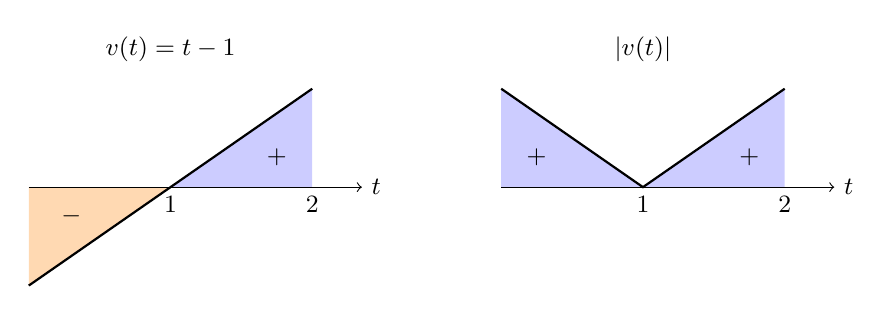
\begin{tikzpicture}[x=1.8cm,y=1.25cm,font=\small]
\begin{scope}
\fill[orange!30] (0,0)--(0,-1)--(1,0)--cycle;
\fill[blue!20] (1,0)--(2,1)--(2,0)--cycle;
\draw[->] (0,0)--(2.35,0) node[right] {$t$};
\draw[thick] (0,-1)--(2,1);
\node at (1,1.4) {$v(t)=t-1$};
\node at (.3,-.3) {$-$};\node at (1.75,.3) {$+$};
\node[below] at (1,0) {$1$};\node[below] at (2,0) {$2$};
\end{scope}
\begin{scope}[xshift=6cm]
\fill[blue!20] (0,0)--(0,1)--(1,0)--(2,1)--(2,0)--cycle;
\draw[->] (0,0)--(2.35,0) node[right] {$t$};
\draw[thick] (0,1)--(1,0)--(2,1);
\node at (1,1.4) {$|v(t)|$};
\node at (.25,.3) {$+$};\node at (1.75,.3) {$+$};
\node[below] at (1,0) {$1$};\node[below] at (2,0) {$2$};
\end{scope}
\end{tikzpicture}
\caption{Displacement adds signed contributions (left), giving zero here.
Distance adds their magnitudes (right), giving one metre.}
\label{fig:velocity-distance}
\end{figure}


\begin{example}[Mass, average value, and accumulated deviation]
If a thin rod occupying \([0,L]\) has continuous linear density
\(\rho(x)\) kilograms per metre, a short piece near $\xi$ has mass
\[
\Delta M\approx\rho(\xi)\Delta x.
\]
Adding the pieces and taking the tagged-sum limit gives total mass
\[
M=\int_0^L\rho(x)\,\dd x.
\]
The dimensional check is
\[
(\text{mass/length})(\text{length})=\text{mass}.
\]
For continuous $f$ on $[a,b]$, its average is the constant $c$ producing
the same total accumulation:
\[
\int_a^b c\,\dd x=\int_a^b f(x)\,\dd x,
\qquad c(b-a)=\int_a^b f(x)\,\dd x.
\]
Dividing by interval length gives
\[
f_{\mathrm{avg}}=\frac1{b-a}\int_a^b f(x)\,\dd x;
\]
the mean value theorem for integrals says this average is attained at some
point. For two continuous profiles $f,g$, the local magnitude of discrepancy is
approximately
\[
|f(\xi_i)-g(\xi_i)|\Delta x_i.
\]
Thus the nonnegative quantity
\[
\int_a^b|f(x)-g(x)|\,\dd x
\]
measures total accumulated vertical deviation, whereas

\[
\int_a^b(f-g)
\]
 permits positive and negative discrepancies to cancel.
In each application, translate the assumptions, choose the
integrand and bounds, check continuity, compute, and interpret the units.
\end{example}

\paragraph{Standard and extended Newton--Leibniz hypotheses.}
The familiar theorem and the next proposition differ only in the regularity
required of the derivative:
\[
\begin{array}{c|c}
\text{standard continuous-derivative setting}
&\text{integrable-derivative extension}\cr\hline
F'\text{ continuous}&F'\text{ merely Riemann integrable}\cr
F\text{ essentially }C^1&F\text{ merely differentiable}\cr
\text{Newton--Leibniz holds}&\text{Newton--Leibniz still holds}.
\end{array}
\]
Thus continuous differentiability is a convenient sufficient hypothesis,
not the boundary of the theorem.

\begin{proposition}[Newton--Leibniz with an integrable derivative]
\label{prop:newton-leibniz-integrable}
If $F$ is continuous on $[a,b]$, differentiable on $(a,b)$, and $F'$
extends to a Riemann-integrable function $g$ on $[a,b]$, then

\[
F(b)-F(a)=\int_a^b g.
\]

\end{proposition}
\begin{proof}
On each partition interval the mean value theorem supplies an interior tag
$\xi_i$ with $F(x_i)-F(x_{i-1})=g(\xi_i)(x_i-x_{i-1})$.
These tags may depend on the partition. Their tagged sum is exactly
\[
S(g,P,\xi)=\sum_i g(\xi_i)(x_i-x_{i-1})
 =\sum_i\bigl(F(x_i)-F(x_{i-1})\bigr)=F(b)-F(a).
\]
Take, for example, equal subdivisions with mesh
\[
(b-a)/N\to0.
\]

By \cref{thm:tagged-riemann}, these particular tagged sums converge
to
\[
\int_a^b g,
\]
 since $g$ is integrable and the theorem allows every
choice of tags. They all equal $F(b)-F(a)$, proving the identity.
\end{proof}

After the measure-zero theory and Lebesgue criterion in section~9.6,
we return to Newton--Leibniz when the derivative identity has a small
exceptional set; see ``\nameref{sec:extended-newton-leibniz}''

\section{Improper Integrals}

For a nonnegative time rate $r$, first distinguish the amount accumulated
by a finite time from a proposed infinite-time total:
\[
A(T)=\int_0^T r(t)\,\dd t,
\qquad A(\infty)=\int_0^\infty r(t)\,\dd t.
\]
The second expression will mean the limit of the first, provided it is
finite. When it is finite, the amount remaining after time $T$ is the tail
\[
A(\infty)-A(T)=\int_T^\infty r(t)\,\dd t.
\]
The finite truncation is the modeled amount before any improper limit is taken.


Finite-interval Riemann integration does not directly cover infinite domains
or unbounded behavior.  Improper integrals retain the finite theory and add
an explicit limiting process whose convergence must be established.

\begin{definition}[Improper Riemann integral]
Let $f:[a,\infty)\to\R$ be Riemann integrable on every finite interval $[a,b]$. The \textbf{improper integral} of $f$ converges if
\[
\int_a^{\infty}f(x)\,\dd x
=\lim_{b\to\infty}\int_a^b f(x)\,\dd x
\]
exists as a finite real number. Define an improper integral at a finite endpoint analogously by a one-sided limit.
\end{definition}

Thus an improper integral is not a new kind of finite-interval integral: it is a limit of ordinary Riemann integrals whose existence must be proved.

\begin{theorem}[Cauchy criterion for improper integrals]
\label{thm:improper-cauchy}
The improper integral $\int_a^\infty f$ converges if and only if, for every
$\eps>0$, there is $A>a$ such that
\[
d>c>A\quad\Longrightarrow\quad
\left|\int_c^d f(x)\,\dd x\right|<\eps.
\]
At a finite singular endpoint, $\int_a^b f$ converges from the right if
and only if, for every $\eps>0$, some $\delta>0$ satisfies
\[
a<c<d<a+\delta\quad\Longrightarrow\quad
\left|\int_c^d f(x)\,\dd x\right|<\eps.
\]
\end{theorem}
\begin{proof}
For the infinite endpoint, put $F(t)=\int_a^t f$. Additivity gives
\[
F(d)-F(c)=\int_c^d f.
\]
Thus the displayed condition is exactly the Cauchy criterion for the real
limit of $F(t)$ as $t\to\infty$. The finite-endpoint statement is the same
argument for the truncation function $F(c)=\int_c^b f$ as $c\to a^+$.
\end{proof}
This is the integral analogue of the series tail criterion:
\[
\sum_{n=N+1}^M a_n\quad\longleftrightarrow\quad\int_c^d f.
\]

At a singular left endpoint, the definition is
\[
\int_a^b f(x)\,\dd x
=\lim_{c\to a^+}\int_c^b f(x)\,\dd x,
\]
when this limit exists finitely; a right-endpoint singularity is analogous.
An interior singularity at $c$ requires two separately convergent integrals,
\[
\int_a^c f+\int_c^b f,
\]
and cancellation between divergent sides is not allowed.  Likewise,
\[
\int_{-\infty}^{\infty}f
=\int_{-\infty}^{c}f+\int_c^{\infty}f
\]
means that both one-sided improper integrals converge, independently of the
chosen finite splitting point $c$.  Infinity is never an endpoint in $\R$.

\begin{example}[$p$-integrals at infinity and at zero]
For real $p$, direct evaluation of the truncated proper integrals gives
\[
\int_1^\infty x^{-p}\,\dd x
\text{ converges exactly when }p>1,
\]
whereas
\[
\int_0^1 x^{-p}\,\dd x
\text{ converges exactly when }p<1.
\]
In particular,
\[
\int_0^1\frac{1}{\sqrt{x}}\,\dd x
=\lim_{c\to0^+}2(1-\sqrt c)=2,
\]
while
\[
\int_0^1x^{-1}\,\dd x,\qquad \int_1^\infty x^{-1}\,\dd x
\]
 diverge.
The opposite thresholds are a useful reminder to identify which endpoint
causes the improper behavior.
\end{example}

The $p$-integral classifications follow from the explicit truncations
\[
\int_1^b x^{-p}\,\dd x=
\begin{cases}\dfrac{b^{1-p}-1}{1-p},&p\ne1,\\\log b,&p=1,\end{cases}
\]
\[
\int_c^1 x^{-p}\,\dd x=
\begin{cases}\dfrac{1-c^{1-p}}{1-p},&p\ne1,\\-\log c,&p=1.\end{cases}
\]
For $p>1$ the first limit is
\[
1/(p-1);
\]
 for $p<1$ the second
is
\[
1/(1-p).
\]
 The other cases diverge to $+\infty$.
Here real powers are available from Chapter~\ref{ch:differentiation}.
Locate each source of impropriety, split at interior singularities, and
truncate each piece. Evaluate the resulting proper integrals and take their
limits independently; convergence requires all of those limits to exist.
The computational choice occurs only after truncation:
\[
\begin{array}{c}
\text{improper integral}\\
\downarrow\\
\text{truncate or split}\\
\downarrow\\[-1mm]
\begin{cases}
\text{easy antiderivative}&\longrightarrow\text{compute and take the limit},\\
\text{substitution, parts, or fractions}
&\longrightarrow\text{transform, compute, and take the limit},\\
\text{no useful closed form}&\longrightarrow\text{comparison or limit comparison}.
\end{cases}
\end{array}
\]

\begin{example}[Ordinary techniques inside improper integrals]
Substitution evaluates
\[
\int_0^\infty xe^{-x^2}\,\dd x
=\lim_{b\to\infty}\int_0^b xe^{-x^2}\,\dd x
=\frac12\lim_{b\to\infty}\int_0^{b^2}e^{-u}\,\dd u
=\frac12.
\]
Integration by parts is applied before the limit:
\[
\int_1^\infty xe^{-x}\,\dd x
=\lim_{b\to\infty}\left([-xe^{-x}]_1^b+
\int_1^b e^{-x}\,\dd x\right)=\frac2e.
\]
Partial fractions give
\[
\int_1^\infty\frac{\dd x}{x(x+1)}
=\lim_{b\to\infty}
\left[\log x-\log(x+1)\right]_1^b
=\log2.
\]
In each calculation the finite truncation is a proper integral and only its
evaluated value is sent to the improper endpoint.
\end{example}

\begin{definition}[Absolute convergence of an improper integral]
An improper integral of $f$ is \textbf{absolutely convergent} if the
corresponding improper integral of $\abs f$ converges.
\end{definition}
\begin{proposition}[Absolute convergence implies convergence]\label{prop:absolute-improper}
If $f$ is integrable on every finite truncation and its improper integral
converges absolutely, then its improper integral converges.
\end{proposition}
\begin{proof}
By the Cauchy criterion applied to $|f|$, for every $\eps>0$ there is
$A$ such that $d>c>A$ implies
\[
\left|\int_c^d f\right|\leq\int_c^d|f|<\eps.
\]
The criterion for $f$ now proves convergence. Finite-endpoint and multiple
improper-endpoint cases are handled one side at a time in the same way.
\end{proof}

\begin{theorem}[Comparison for improper integrals]
\label{thm:improper-comparison}
Let $0\leq f\leq g$ on $[a,\infty)$, with both functions Riemann integrable on finite intervals. If the improper integral of $g$ converges, then that of $f$ converges.
\end{theorem}
\begin{proof}
Put
\[
H(b)=\int_a^b f.
\]
 Nonnegativity makes $H$ increasing in its
real endpoint $b$, and comparison bounds it by the finite improper
integral of $g$. Set $L=\sup\{H(b):b\geq a\}$. Given $\eps>0$,
choose $c$ with $H(c)>L-\eps$. For every real $b\geq c$,

\[
L-\eps<H(c)\leq H(b)\leq L.
\]
 This is $H(b)\to L$ as $b\to\infty$;
the monotone-convergence argument applies, now with
a real endpoint rather than an integer index.
\end{proof}

\begin{corollary}[Limit comparison for improper integrals]
Let $f,g:[a,\infty)\to\R$ be Riemann integrable on every finite interval
$[a,b]$. Suppose $f,g>0$ eventually and
\[
\lim_{x\to\infty}\frac{f(x)}{g(x)}=L,
\qquad0<L<\infty.
\]
Then their improper integrals have the same convergence behavior.
\end{corollary}
\begin{proof}
Choose $A_0$ from which $f,g>0$, and $A_1$ such that

\[
|f(x)/g(x)-L|<L/2
\]
 for $x>A_1$. For every
$x>A=\max\{A_0,A_1,a\}$,
\[
(L/2)g(x)<f(x)<(3L/2)g(x).
\]

Apply comparison on that tail in both directions;
changing a finite initial interval does not affect convergence.
\end{proof}

\begin{example}[Comparison instead of an antiderivative]
On $[1,\infty)$,
\[
0\leq1/(1+x^2)\leq1/x^2,
\]
 so its improper
integral converges. For
\[
(2x+1)/(x^3+1),
\]
 the ratio to
\[
1/x^2
\]

tends to $2$; positive limit comparison gives convergence.
For
\[
1/\sqrt{x^2+1},
\]
 the ratio to
\[
1/x
\]
 tends to $1$;
its integral diverges. All integrands are continuous on finite
truncations. These tests decide existence without requiring a formula
for the accumulated value.
\end{example}

\begin{example}[An infinite-time accumulation]
A device releases material at rate
\[
r(t)=2/(1+t)^2
\]
 grams per hour
for $t\geq0$. The assumptions specify the rate at every nonnegative
time. The amount released by time $b$ is
\[
A(b)=\int_0^b\frac{2}{(1+t)^2}\,\dd t
=2-\frac{2}{1+b}\quad\text{grams}.
\]
Therefore the infinite-time total is $2$ grams, defined as the
improper limit. The amount yet to be released after time $b$ is

\[
2/(1+b)
\]
 grams, below a tolerance $\eta>0$ when
\[
b>2/\eta.
\]

The formula yields both a finite limiting total and a usable error bound.
\end{example}

We now close the logical gap explicitly marked in
\cref{rem:integral-test-preview}: proper integrals, their improper
limits, and the needed comparison principles have all been established.
The preview's rectangle argument can now be a proof.

\begin{theorem}[Integral test]
\label{thm:integral-test}
Let $f:[1,\infty)\to\R$ be continuous, nonnegative, and decreasing, and put $a_n=f(n)$. Then
\[
\sum_{n=1}^{\infty}a_n
\]
converges if and only if the improper integral
\[
\int_1^{\infty}f(x)\,\dd x
\]
converges. More precisely, for every $N\in\N$,
\[
\int_1^{N+1}f(x)\,\dd x
\leq\sum_{n=1}^{N}f(n)
\leq f(1)+\int_1^{N}f(x)\,\dd x.
\]
\end{theorem}
\begin{proof}
For $x\in[n,n+1]$, monotonicity gives
\[
f(n+1)\leq f(x)\leq f(n).
\]
Integrating these inequalities over the unit intervals and summing gives the displayed bounds. The partial sums and truncated integrals are increasing, so each is bounded above if and only if the other is bounded above. For real endpoints, if $b\geq1$, choose an integer $N\geq b$;
then
\[
\int_1^b f\leq\int_1^N f.
\]
 Thus boundedness at integer
endpoints is boundedness at all endpoints. The supremum argument in
\cref{thm:improper-comparison} proves convergence of these increasing
truncations; monotone convergence proves convergence of the partial sums.
This proves the equivalence for the genuine improper limit.
\end{proof}

\begin{theorem}[$p$-series test: analytic rederivation]
\label{thm:p-series-test}
For $p\in\R$, the series
\[
\sum_{n=1}^{\infty}\frac{1}{n^p}
\]
converges if and only if $p>1$.
\end{theorem}
\begin{proof}
For rational $p$, this conclusion was already proved without integration in \cref{thm:rational-p-series-test}. We now give an analytic proof that extends the criterion to every real exponent, using the real powers constructed in Chapter~\ref{ch:differentiation}.

For $p>0$, the function
\[
f(x)=x^{-p}
\]
is continuous, nonnegative, and decreasing on $[1,\infty)$ by \cref{thm:real-power-derivative}. If $p\ne1$, that theorem gives
\[
\frac{\dd}{\dd x}\left(\frac{x^{1-p}}{1-p}\right)=x^{-p};
\]
if $p=1$, \cref{thm:log-and-inverses} gives
\[
\frac{\dd}{\dd x}\log x=\frac1x.
\]
Thus \cref{thm:ftc-two} gives
\[
\int_1^b x^{-p}\,\dd x=
\begin{cases}
\dfrac{b^{1-p}-1}{1-p},&p\ne1,\\
\log b,&p=1.
\end{cases}
\]
Thus the improper integral converges exactly when $p>1$, and \cref{thm:integral-test} gives the conclusion. If $p\leq0$, the terms do not tend to zero, so the series diverges by \cref{prop:series-terms-zero}.
\end{proof}

\begin{example}[Cancellation at a singularity]
The two one-sided integrals of
\[
1/x
\]
 across zero diverge: the negative
side gives $\log\delta\to-\infty$, the positive side gives
$-\log\eta\to+\infty$. Choosing $\delta=\eta$ cancels them at each
stage but does not define an improper integral. That linked-cutoff limit
is a Cauchy principal value. Choosing $\eta=\delta^2$ instead makes
the sum $-\log\delta$ diverge. Independent one-sided convergence is essential.
\end{example}
\section{The Lebesgue Criterion for Riemann Integrability}

Continuity is sufficient for Riemann integrability, but it is not necessary.
The natural question is how large a discontinuity set Riemann integration can
tolerate.  Darboux sums measure oscillation on intervals; the criterion below
answers the question by asking whether discontinuities fit inside interval
covers of arbitrarily small total length.  This will make the
Dirichlet--Thomae comparison decisive: density alone does not decide
integrability.  We use only countable interval covers, not a formal theory of
Lebesgue measure.

For comparison, \cref{thm:monotone-discontinuities} already proves that a
monotone function has at most countably many discontinuities. The direct
Darboux proof of monotone integrability earlier in this chapter remains
logically independent of the criterion developed here.

Ordinary interval length is the starting point for Lebesgue measure \(\mu\),
which assigns a generalized length to a large class of subsets of $\R$,
called measurable sets. Not every subset of $\R$ is measurable. Ordinary
intervals are measurable, and for \(a<b\),
\[
\boxed{
\mu([a,b])=\mu((a,b))=\mu([a,b))=\mu((a,b])=b-a.}
\]
Indeed, \(\mu(\{a\})=\mu(\{b\})=0\), so adding or deleting finitely many
endpoints does not change measure.
The central property, stated here without proof, is countable additivity:
for pairwise disjoint measurable sets $E_j$,
\[
\mu\!\left(\bigcup_{j=1}^{\infty}E_j\right)
=\sum_{j=1}^{\infty}\mu(E_j).
\]
Lebesgue measure is also \emph{translation invariant}, a fact stated
without proof: for every measurable $E\subseteq\R$ and $t\in\R$, the
translate is measurable and
\[
E+t=\{x+t:x\in E\},\qquad \mu(E+t)=\mu(E).
\]
Translation preserves length; it does not remove overlap. For example,
\[
E=[0,1],\qquad F=E+\frac12,
\]
have equal measure by translation invariance, but
\[
\mu(E)+\mu(F)=2,\qquad \mu(E\cup F)=\frac32.
\]
The overlap has been counted twice in the sum. Pairwise disjointness in
countable additivity ensures that no portion is counted more than once.
A standard consequence of countable additivity, also used here without
proof, is countable subadditivity:
\[
\mu\!\left(\bigcup_{j=1}^{\infty}E_j\right)
\leq\sum_{j=1}^{\infty}\mu(E_j).
\]
Thus, if a measurable set $E$ is covered by open intervals $I_j$ of total
length less than $\varepsilon$, then
\[
\begin{aligned}
\mu(E)&\leq \mu\!\left(\bigcup_{j=1}^{\infty}I_j\right)
\leq\sum_{j=1}^{\infty}\mu(I_j)\\
&=\sum_{j=1}^{\infty}\ell(I_j)<\varepsilon.
\end{aligned}
\]
If such a cover exists for every $\varepsilon>0$, then \(\mu(E)=0\).
A theorem of Lebesgue measure theory, also stated without proof, says that
\emph{all} subsets satisfying this interval-cover condition are measurable
and have measure zero, and conversely every measure-zero set has such covers.
We can therefore use the following self-contained covering definition.
Only this property is used in this chapter; neither a construction of
Lebesgue measure nor Lebesgue integration is required.

A discontinuity need not be a jump. To measure all possible local failures
of continuity at once, compare every pair of nearby values and then shrink
the neighborhood. The resulting oscillation records the variation that
cannot be removed by choosing a smaller neighborhood.

\begin{definition}[Oscillation and measure-zero sets]
Let $f:[a,b]\to\R$ be bounded.  For each $x\in[a,b]$, define
\[
N_\delta(x)=[a,b]\cap(x-\delta,x+\delta),
\qquad
\boxed{\omega_f(x)=\inf_{\delta>0}
\operatorname{osc}_{N_\delta(x)}(f).}
\]
Shrinking the neighborhood can only decrease its oscillation by restriction
monotonicity. Thus $\omega_f(x)$ is the variation that cannot be removed by
zooming in at $x$.
A set $E\subseteq[a,b]$ has \textbf{Lebesgue measure zero} if, for every $\eta>0$, there are open intervals $I_1,I_2,\ldots$ such that
\[
E\subseteq\bigcup_{j=1}^{\infty}I_j
\qquad\text{and}\qquad
\sum_{j=1}^{\infty}\ell(I_j)<\eta.
\]
Finite covers are allowed as a special case.
\end{definition}

\begin{remark}[Null sets and almost everywhere]
A measure-zero set is also called a \emph{null set}. A property holds
\emph{almost everywhere} (a.e.) if it holds outside a set of Lebesgue
measure zero.
\end{remark}

\begin{proposition}[Oscillation and continuity]
\label{prop:oscillation-continuity}
Let $f:[a,b]\to\R$ be bounded.  Then
\[
\omega_f(x)=0
\]
if and only if $f$ is continuous at $x$.
\end{proposition}
\begin{proof}
If $f$ is continuous at $x$, then, for a given $\varepsilon>0$, all values
in a sufficiently small relative neighborhood of $x$ lie within

\[
\varepsilon/2
\]
 of $f(x)$.  Their pairwise differences are therefore less
than $\varepsilon$, since
\[
|f(y)-f(z)|\leq|f(y)-f(x)|+|f(z)-f(x)|.
\]
Thus the defining infimum is zero. Conversely, if
$\omega_f(x)=0$, then the defining infimum supplies a $\delta>0$ for which
the pairwise oscillation in the relative $\delta$-neighborhood of $x$ is
less than $\varepsilon$.  Taking one of the two points to be $x$ gives
\[
\lvert f(y)-f(x)\rvert<\varepsilon
\]
whenever $\lvert y-x\rvert<\delta$.
\end{proof}

\begin{proposition}[Closed oscillation sets]
\label{prop:closed-oscillation-sets}
Let $f:[a,b]\to\R$ be bounded and let $\varepsilon>0$.  Then
\[
D_{\varepsilon}=\bigl\{x\in[a,b]:\omega_f(x)\geq\varepsilon\bigr\}
\]
is closed in $[a,b]$.
\end{proposition}
\begin{proof}
If $\omega_f(x)<\varepsilon$, choose $r>0$ with
\[
\operatorname{osc}_{N_r(x)}(f)<\varepsilon.
\]
If $|y-x|<r/2$, then $N_{r/2}(y)\subseteq N_r(x)$, and hence
\[
\omega_f(y)\leq\operatorname{osc}_{N_{r/2}(y)}(f)
\leq\operatorname{osc}_{N_r(x)}(f)<\varepsilon.
\]
Hence the complement of
$D_{\varepsilon}$ is open.
\end{proof}

\begin{proposition}[Countable sets have measure zero]
\label{prop:countable-negligible}
Every countable subset of $[a,b]$ has measure zero.
\end{proposition}
\begin{proof}
Let
\[
E\subseteq\{x_1,x_2,\ldots\},
\]
where repetitions are allowed if $E$ is finite.  Given $\eta>0$, cover
$x_n$ by an open interval of length
\[
\frac{\eta}{2^{n+1}}.
\]
These intervals cover $E$, and their total length is less than $\eta$.
\end{proof}

\begin{lemma}[Countable unions of measure-zero sets]
\label{lem:countable-union-negligible}
If
\[
E_1,E_2,\ldots\subseteq[a,b]
\]
have measure zero, then
\[
\bigcup_{m=1}^{\infty}E_m
\]
has measure zero.
\end{lemma}
\begin{proof}
Given $\eta>0$, cover $E_m$ by open intervals having total length less
than
\[
\frac{\eta}{2^{m+1}}.
\]
The combined doubly indexed family is countable by the countability result
of Chapter~2, covers the displayed union, and has total length less than
$\eta$.
\end{proof}

The criterion uses two error accounts. On good intervals the oscillation
is small, even if their total length is large. On bad intervals the
oscillation may be large, but their total length must be small.
\[
\underbrace{\sum_{\rm good}\operatorname{osc}_I(f)|I|}_{\leq\eta(b-a)}
+\underbrace{\sum_{\rm bad}\operatorname{osc}_I(f)|I|}_{\leq2M\,\ell_{\rm bad}}.
\]
With $|f|\leq M$, choose
\[
\eta(b-a)<\eps/2,\qquad 2M\ell_{\rm bad}<\eps/2.
\]
 Large oscillation is acceptable when
confined to intervals of sufficiently small combined length.
\begin{center}
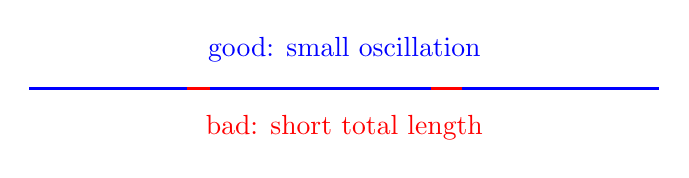
\begin{tikzpicture}
\draw[thick] (0,0)--(8,0);
\draw[blue,very thick] (0,0)--(2,0) (2.3,0)--(5.1,0) (5.5,0)--(8,0);
\draw[red,very thick] (2,0)--(2.3,0) (5.1,0)--(5.5,0);
\node[blue] at (4,.5) {good: small oscillation};
\node[red] at (4,-.5) {bad: short total length};
\end{tikzpicture}
\end{center}
\begin{theorem}[Lebesgue criterion for Riemann integrability]
\label{thm:riemann-lebesgue-criterion}
Let $f:[a,b]\to\R$ be bounded. Then
\[
\boxed{f\text{ is Riemann integrable}
\iff \operatorname{Disc}(f)\text{ has Lebesgue measure zero}.}
\]
Here $\operatorname{Disc}(f)$ denotes the discontinuity set. For the proof,
we use the following equivalent formulations.
\begin{enumerate}
\item $f$ is Riemann integrable.
\item For every $\varepsilon>0$, the set
\[
D_{\varepsilon}=\bigl\{x\in[a,b]:\omega_f(x)\geq\varepsilon\bigr\}
\]
has measure zero.
\item The discontinuity set of $f$ has measure zero.
\end{enumerate}
\end{theorem}
\begin{remark}[Terminology]
This result is commonly called \textbf{Lebesgue's criterion for Riemann
integrability}.  Some sources use a name such as the
\textbf{Riemann--Lebesgue criterion}; it must not be confused with the
Riemann--Lebesgue lemma from Fourier analysis.
\end{remark}
\begin{proof}
\textbf{(a)$\Rightarrow$(b): small gap forces short large-oscillation
cells.} Fix an oscillation threshold $\alpha>0$ and a cover budget
$\eta>0$. By the Darboux criterion choose $P$ with
$U(f,P)-L(f,P)<\alpha\eta/4$. Then
\[
\alpha\sum_{\operatorname{osc}_{I_i}(f)\geq\alpha}\ell(I_i)
\leq\sum_{\operatorname{osc}_{I_i}(f)\geq\alpha}
\operatorname{osc}_{I_i}(f)\ell(I_i)
\leq U(f,P)-L(f,P).
\]
Thus the large-oscillation cells have combined length below $\eta/4$.
Every non-partition point $x\in D_\alpha$ lies in the interior of one such
cell: otherwise a small relative neighborhood of $x$ inside its cell would
have oscillation below $\alpha$, contradicting
$\omega_f(x)\geq\alpha$. Enlarge the finitely many large cells slightly to
open intervals of total length below $\eta/2$, and cover the finitely many
partition points separately with total length below $\eta/2$. This covers
$D_\alpha$ within budget $\eta$.

\textbf{(b)$\Rightarrow$(a): four stages.} Fix $\eps>0$ and choose
$M\geq1$ with $|f|\leq M$.

\emph{Stage 1: choose the vertical threshold.} Select $\alpha>0$ so that
\[
\alpha(b-a)<\eps/2.
\]

\emph{Stage 2: make the bad cover short and finite.} Cover $D_\alpha$ by
open intervals with total length below $\eps/(4M)$. The set $D_\alpha$ is
relatively closed by \cref{prop:closed-oscillation-sets}, hence compact by
\cref{cor:closed-subset-finite-subcover}; retain a finite subcover and let
$O$ be its union.

\emph{Stage 3: obtain one common horizontal scale.} For each
$x\in[a,b]\setminus O$, the inequality $\omega_f(x)<\alpha$ supplies an
open interval $V_x$ on which $\operatorname{osc}(f)<\alpha$. The finitely
many bad intervals together with the $V_x$ cover $[a,b]$. Apply
\cref{lem:lebesgue-number-interval} and choose $P$ with
$\operatorname{mesh}(P)<\lambda$.

\emph{Stage 4: split the Darboux gap.} A cell is bad if it lies in one of
the selected bad intervals; every other cell lies in some $V_x$ and is
good. Assigning each bad cell to one selected interval shows that their
combined length is below $\eps/(4M)$. Therefore
\[
\begin{aligned}
U(f,P)-L(f,P)
&=\sum_{\text{good }I}\operatorname{osc}_I(f)\ell(I)
 +\sum_{\text{bad }I}\operatorname{osc}_I(f)\ell(I)\\
&<\alpha(b-a)+2M\frac{\eps}{4M}<\eps.
\end{aligned}
\]
The Darboux criterion proves (a).

Finally, \cref{prop:oscillation-continuity} and the Archimedean property
give
\[
\operatorname{Disc}(f)=\bigcup_{m=1}^\infty D_{1/m}.
\]
Indeed, discontinuity is equivalent to $\omega_f(x)>0$, and then some
$m$ satisfies $1/m\leq\omega_f(x)$. Countable-union stability proves
(b)$\Rightarrow$(c), while $D_\alpha\subseteq\operatorname{Disc}(f)$
proves (c)$\Rightarrow$(b).
\end{proof}

\begin{example}[The Dirichlet function]
\label{ex:dirichlet-function}
For
\[
\mathbf{1}_{\mathbb{Q}}:[0,1]\to\R,
\]
every neighborhood contains rational and irrational points.  Hence
\[
\omega_{\mathbf{1}_{\mathbb{Q}}}(x)=1
\qquad(x\in[0,1]),
\]
so
\[
D_{1/2}=[0,1]
\]
does not have measure zero.
\end{example}

\begin{example}[Thomae's function]
\label{ex:thomae-function}
For $x\in[0,1]$, define
\[
T(x)=
\begin{cases}
1/q,&x=p/q\text{ is rational and written in lowest terms},\\
0,&x\text{ is irrational}.
\end{cases}
\]
This is commonly called \textbf{Thomae's function}, or the
\textbf{popcorn function}; some texts call it Riemann's function, a name
best avoided because it is ambiguous in analysis.  The function $T$ is
continuous at every irrational point and discontinuous at every rational
point.  Consequently,
\[
\operatorname{Disc}(T)=\Q\cap[0,1],
\]
$T$ is Riemann integrable, and
\[
\int_0^1T(x)\,\dd x=0.
\]
\end{example}
\begin{proof}
Let $x$ be irrational, and fix $\varepsilon>0$.  There are only finitely
many rational numbers in $[0,1]$ that, in lowest terms, have denominator
\[
q\leq\frac1\varepsilon;
\]
indeed, there are only finitely many possible numerators for each such
denominator.  Let $F_\varepsilon$ be this finite set.  Since
\[
x\notin F_\varepsilon,
\]
there is a neighborhood of $x$ avoiding $F_\varepsilon$.  At every point
$y$ in this neighborhood, either $y$ is irrational and $T(y)=0$, or its
reduced denominator satisfies
\[
q>\frac1\varepsilon,
\]
so
\[
T(y)=\frac1q<\varepsilon.
\]
Since $T(x)=0$, this proves that $T$ is continuous at $x$.

If
\[
x=p/q\in[0,1]
\]
 is rational in lowest terms, irrational density
(\cref{prop:irrational-density}) supplies an irrational point in every
relative open neighborhood of $x$. There $T$ is zero, whereas
\[
T(x)=1/q.
\]

The continuity test with
\[
\eps=1/(2q)
\]
 therefore fails at $x$, including
at the endpoints. This proves the stated discontinuity set.

The set
\[
\Q\cap[0,1]
\]
is countable and therefore has measure zero by
\cref{prop:countable-negligible}.  The criterion proves that $T$ is
integrable.  Finally, every nondegenerate subinterval of $[0,1]$ contains an
irrational point by \cref{prop:irrational-density}.
The infimum of $T$ on it is therefore zero.  Every lower Darboux sum is zero;
since $T$ is integrable, its integral is zero.
\end{proof}

\begin{remark}[The Dirichlet--Thomae contrast]
Earlier integrability proofs constructed partitions and estimated
\[
U(f,P)-L(f,P).
\]
The criterion often saves that work: identify the discontinuity set, show
it has measure zero, and conclude integrability. A direct Darboux proof for
Thomae's function requires separating the finitely many large values from
the small ones. Once continuity has been analyzed, the criterion gives
\[
\operatorname{Disc}(T)=\Q\cap[0,1],
\]
a countable set, hence a set of measure zero. Thus $T$ is Riemann integrable.
For the Dirichlet function,
\[
\operatorname{Disc}(\mathbf1_{\Q})=[0,1],\qquad \mu([0,1])=1,
\]
so it is not Riemann integrable. Density alone does not determine
integrability; the measure-theoretic size of the discontinuity set does.
\end{remark}




\subsection{How Far Can Newton--Leibniz Be Extended?}
\label{sec:extended-newton-leibniz}

Three separate assertions enter the Fundamental Theorem of Calculus:
\[
\boxed{F\text{ is differentiable},\qquad
f\text{ is Riemann integrable},\qquad F'=f.}
\]
The first concerns the existence of a local rate of change, the second
the convergence of sums, and the third identifies two functions. Neither
of the first two assertions alone gives the other assertions.
In the finite- and countable-exception theorems below, $F'$ exists at every
interior point; only the identity $F'=f$ is allowed to fail on the stated
exceptional set. This differs from the later Lipschitz/a.e. theorem, where
differentiability itself may fail on a null set.

\begin{example}[Differentiable need not mean \(C^1\)]
\label{ex:bounded-discontinuous-derivative}
Set
\[
F(0)=0,
\qquad
F(x)=x^2\sin(1/x)\quad(x\ne0).
\]
Then
\[
|F(h)/h|\leq|h|,
\]
 so \(F'(0)=0\), while for \(x\ne0\),
\[
F'(x)=2x\sin(1/x)-\cos(1/x).
\]
This derivative is bounded near zero but has no limit there. Hence \(F\) is
differentiable and is not \(C^1\). On every compact interval, \(F'\) is
bounded and continuous except at zero, so the finite-discontinuity argument
following \cref{thm:tagged-riemann} makes it Riemann integrable.
Consequently,
\[
F'\text{ Riemann integrable}
\not\Longrightarrow
F'\text{ continuous},
\]
and \cref{prop:newton-leibniz-integrable} is genuinely stronger than the
continuous-derivative version of the FTC.
\end{example}

\begin{example}[A Riemann-integrable jump is not a derivative]
Let \(j(x)=0\) for \(x<0\) and \(j(x)=1\) for \(x\geq0\) on
\([-1,1]\). This bounded monotone function is Riemann integrable. It cannot
equal \(F'\) everywhere for any differentiable \(F\), because derivatives
have the intermediate value property by \cref{thm:darboux-derivatives}, while
\(j\) omits every value strictly between \(0\) and \(1\). Thus
\[
\text{Riemann integrable}
\not\Longrightarrow
\text{is a derivative}.
\]
\end{example}

\begin{example}[A differentiable function with an unbounded derivative]
\label{ex:unbounded-derivative}
Set $F(0)=0$ and
\[
F(x)=x^2\sin(1/x^2)
\]
 for $x\ne0$. Since
\[
\left|\frac{F(h)-F(0)}h\right|=|h\sin(1/h^2)|\leq |h|\longrightarrow0,
\]
we have $F'(0)=0$. At other points,
\[
F'(x)=2x\sin(1/x^2)-\frac2x\cos(1/x^2).
\]
For
\[
x_n=(2\pi n)^{-1/2},
\]
 one has $F'(x_n)=-2\sqrt{2\pi n}$.
The sequence $-x_n$ gives the corresponding positive values. Thus $F'$
is unbounded on every nondegenerate compact interval containing zero,
even if zero is an endpoint, and is not Riemann integrable there:
\[
F\text{ differentiable}\ \not\Longrightarrow\ F'\text{ Riemann integrable}.
\]
\end{example}

\begin{example}[An accumulation function with a corner]
\label{ex:step-accumulation}
On $[-1,1]$ let $f(x)=0$ for $x<0$ and $f(x)=1$ for $x\geq0$.
This monotone function is Riemann integrable, and direct integration gives
\[
A(x)=\int_{-1}^x f(t)\,\dd t
=\begin{cases}0,&-1\leq x\leq0,\\x,&0\leq x\leq1.\end{cases}
\]
The left derivative of $A$ at zero is $0$, while the right derivative is
$1$. The accumulation-function theorem guarantees $A'=f$ at continuity
points of $f$; it makes no such promise at its jump. In particular,
\[
f\text{ Riemann integrable}\ \not\Longrightarrow\
\left(\int_a^x f\right)'=f\text{ everywhere}.
\]
\end{example}

\begin{lemma}[Finite modifications]
\label{lem:finite-modifications}
If bounded functions $f,g:[a,b]\to\R$ differ only at finitely many points
and $f$ is Riemann integrable, then $g$ is Riemann integrable and
\[
\int_a^b g=\int_a^b f.
\]
\end{lemma}
\begin{proof}
Put $u=g-f$. Then $u=0$ off a finite set $E$ and $|u|\leq B$ for some
$B$. Surround the points of $E$ by intervals of arbitrarily small total
length and insert their endpoints in a partition. Every other cell has
zero oscillation, while each bad cell has oscillation at most $2B$.
Consequently the Darboux gap for $u$ can be made arbitrarily small, so $u$
is integrable. Moreover both $|L(u,P)|$ and $|U(u,P)|$ are at most $B$
times the total bad length; squeezing gives $\int u=0$. Linearity yields
the conclusion. Endpoint modifications are included.
\end{proof}

\Needspace{12\baselineskip}
\begin{theorem}[Newton--Leibniz with finitely many exceptions]
\label{thm:ftc-finite-exceptions}
Let $F$ be continuous on $[a,b]$ and differentiable on $(a,b)$, and let
$f:[a,b]\to\R$ be Riemann integrable. If $F'(x)=f(x)$ except at
finitely many points of $(a,b)$, then
\[
\boxed{F(b)-F(a)=\int_a^b f(t)\,\dd t.}
\]
\end{theorem}
\begin{proof}
Replace $f(x)$ by $F'(x)$ at the exceptional interior points, retaining
the endpoint values of $f$. The resulting function is a Riemann-integrable
extension of $F'$ with the same integral as $f$. Apply
\cref{prop:newton-leibniz-integrable}.
\end{proof}

\begin{theorem}[Newton--Leibniz with countably many exceptions]
\label{thm:ftc-countable-exceptions}
Let $F$ be continuous on $[a,b]$ and differentiable on $(a,b)$, and let
$f:[a,b]\to\R$ be Riemann integrable. Suppose $E\subset(a,b)$ is
countable and $F'(x)=f(x)$ for $x\in(a,b)\setminus E$. Then
\[
\boxed{F(b)-F(a)=\int_a^b f(t)\,\dd t.}
\]
\end{theorem}
\begin{proof}
\textbf{Strategy.} Transfer local bounds on $f$ to $F'$ by Darboux's
theorem, then squeeze increments of $F$ between the Darboux sums of $f$.
\medskip

\textbf{Stage 1: transfer local bounds from $f$ to $F'$.}
First let $J\subset(a,b)$ be a nonempty open interval on which
$\alpha\leq f\leq\beta$. We claim that the same bounds hold for $F'$.
If $F'(t_0)>\beta$, choose $s\in J\setminus E$, possible because every
nondegenerate interval is uncountable. Then $F'(s)=f(s)\leq\beta$.
By \cref{thm:darboux-derivatives}, every value in $(\beta,F'(t_0))$
is attained between $s$ and $t_0$, hence inside $J$. All such values
must be attained at exceptional points. This puts an uncountable interval
inside the countable image $F'(E\cap J)$, a contradiction. Apply the
same argument to $-F,-f$ for the lower bound. Thus
\[
\alpha\leq F'(t)\leq\beta\qquad(t\in J).
\]
\textbf{Stage 2: compare increments with Darboux sums.}
For a partition $a=x_0<\cdots<x_n=b$, put
$m_i=\inf_{[x_{i-1},x_i]}f$ and $M_i=\sup_{[x_{i-1},x_i]}f$.
The local bound applies on $(x_{i-1},x_i)$. The Mean Value Theorem,
using continuity of $F$ at the endpoints and differentiability at every
interior point, gives
\[
m_i\Delta x_i\leq F(x_i)-F(x_{i-1})\leq M_i\Delta x_i.
\]
Summing yields
\[
L(f,P)\leq F(b)-F(a)\leq U(f,P).
\]

The integral lies in this same interval; Riemann integrability makes its
length arbitrarily small, proving the equality.
\end{proof}

Finite changes preserve integrability without further assumptions.
Countable changes need not: changing the zero function to $1$ at rational
points produces the Dirichlet function. In the theorem, the changed
function is a derivative. Darboux's property prevents its exceptional
values from escaping the bounds forced by nearby nonexceptional values.
Countability excludes an interval of such values. The local bounds then
place each increment of $F$ between the corresponding lower and upper
Darboux contributions of $f$, so integrability of $f$ completes the proof.

\begin{theorem}[Lipschitz, almost-everywhere Riemann form]
\label{thm:ftc-lipschitz-ae}
Let $F:[a,b]\to\R$ be Lipschitz and let $f:[a,b]\to\R$ be Riemann
integrable. If $F'=f$ almost everywhere on $(a,b)$ (in particular, $F'$ exists
outside a set of Lebesgue measure zero), then
\[
\boxed{F(b)-F(a)=\int_a^b f(t)\,\dd t.}
\]
\end{theorem}
Here \emph{almost everywhere}, abbreviated a.e., means outside a
set of Lebesgue measure zero. This is the strongest form developed here whose
right-hand side remains an ordinary Riemann integral.
The proof is not developed here because it requires the measure-theoretic
structure of Lipschitz functions. For the needed results, see for example
\cite{pugh-analysis,rudin-pma}.
For
\[
A(x)=\int_a^x f(t)\,\dd t,
\]
the integral estimate makes $A$ Lipschitz, and
the accumulation theorem and Lebesgue criterion give $A'=f$ a.e.
Thus $F-A$ is Lipschitz with derivative zero a.e. To conclude that it is
constant requires a deeper theorem about Lipschitz functions; its proof
belongs to measure-theoretic real analysis and is deferred here.

\begin{remark}[The Cantor-function warning]
\label{rem:cantor-ftc-warning}
There exists a continuous nondecreasing function $C:[0,1]\to[0,1]$,
called the Cantor function, with $C(0)=0$, $C(1)=1$, and $C'=0$ almost
everywhere. Its construction is not needed here; see
\cite{abbott-analysis,pugh-analysis} for standard treatments. For $f=0$ it gives
\[
C'=f\text{ a.e.},\qquad \int_0^1 f=0,
\qquad C(1)-C(0)=1.
\]
Continuity together with an a.e. derivative identity therefore does not
suffice for Newton--Leibniz. The Cantor function is not Lipschitz.
This does not show that Lipschitz continuity is the weakest possible
sufficient condition: absolute continuity, defined next, is weaker and
is the condition that characterizes indefinite Lebesgue integrals.
\end{remark}


\section{Limits of the Riemann Theory}

Section~9.6 has already encountered the simplest important
measure-theoretic notion of size: sets of Lebesgue measure zero. Full
measure theory extends this from recognizing null sets to assigning
generalized length systematically and defining a new integral. This leads
to the relation between absolute continuity and integration described below.

The Dirichlet function differs from zero only on the null set
$\Q\cap[0,1]$, yet it is not Riemann integrable. Thus changing a function
on a null set can destroy Riemann integrability. Thomae's function,
whose discontinuity set is the same dense countable set, shows that density
of the discontinuity set alone is not the obstruction. Improper integrals also force one to treat unbounded
behavior and infinite domains by separate limiting conventions.

The resulting progression is:
\[
\boxed{
\begin{gathered}
\text{Riemann integrability}\longrightarrow\text{measure-zero exceptional sets}\\
\longrightarrow\text{Lebesgue measure and integration}\\
\longrightarrow\text{MCT and DCT}\\
\longrightarrow\text{absolute continuity and the Lebesgue FTC}
\end{gathered}}
\]

\subsection*{An informal working framework for Lebesgue integration}
A notion of size is generally assigned not to every subset of a set $X$,
but to a specified collection on which it behaves consistently. Some
measures, including counting measure and the zero measure, can be defined on
all of $\mathcal P(X)$. The obstruction is instead geometric: ordinary
length on $\R$ cannot be extended to every subset while remaining countably
additive, translation invariant, and consistent with interval length, for
example $\mu([0,1])=1$. Lebesgue measure is therefore defined on a large
family of Lebesgue-measurable sets, not on all of $\mathcal P(\R)$.

\begin{definition}[$\sigma$-algebra and measurable space]
For a set $X$, a \emph{$\sigma$-algebra} is a family
$\mathcal A\subseteq\mathcal P(X)$ such that
\[
X\in\mathcal A,
\qquad E\in\mathcal A\Longrightarrow X\setminus E\in\mathcal A,
\]
and
\[
E_1,E_2,\ldots\in\mathcal A
\Longrightarrow \bigcup_{n=1}^\infty E_n\in\mathcal A.
\]
Its members are \emph{measurable sets}, and $(X,\mathcal A)$ is a
\emph{measurable space}. Complements and countable unions repeatedly arise
in limiting arguments, so the admissible sets must remain stable under them.
\end{definition}

\begin{definition}[Measure]
A \emph{measure} on $(X,\mathcal A)$ is a function
\[
\mu:\mathcal A\to[0,\infty]
\]
such that $\mu(\varnothing)=0$ and, for pairwise disjoint measurable sets,
\[
\mu\!\left(\bigcup_{n=1}^\infty E_n\right)
=\sum_{n=1}^\infty\mu(E_n).
\]
\end{definition}

The \emph{Borel $\sigma$-algebra} on the line is
\[
\mathcal B(\R)=\sigma(\{\text{open subsets of }\R\}).
\]
Here ``generated by'' means
\[
\boxed{\mathcal B(\R)\text{ is the smallest $\sigma$-algebra containing
every open subset of }\R.}
\]
Starting with the open sets, one repeatedly closes the family under
complements and countable unions. De Morgan's law also supplies countable
intersections:
\[
\bigcap_{n=1}^\infty E_n
=\left(\bigcup_{n=1}^\infty E_n^c\right)^c.
\]
The word \emph{repeatedly} matters: one round of these operations does not
describe all Borel sets. By \cref{prop:real-open-interval-components}, open
intervals generate the same $\sigma$-algebra. The Lebesgue $\sigma$-algebra
is larger: it contains all Borel sets and all subsets of Lebesgue-null sets.

\begin{definition}[Measurable maps]
A map
\[
f:(X,\mathcal A)\to(Y,\mathcal B)
\]
is \emph{measurable} if $f^{-1}(B)\in\mathcal A$ for every
$B\in\mathcal B$. A real-valued measurable function has target
$(\R,\mathcal B(\R))$.
\end{definition}

\begin{proposition}[Threshold criterion for real-valued measurability]
\label{prop:measurable-threshold-preview}
A real-valued function $f$ on $(X,\mathcal A)$ is measurable if and only if
\[
\{x\in X:f(x)>\alpha\}\in\mathcal A
\qquad\text{for every }\alpha\in\R.
\]
\end{proposition}
The proof is not developed here. The threshold form says concretely that
the region on which $f$ lies above each prescribed level is measurable.
If $X$ is a topological space equipped with its Borel $\sigma$-algebra, every
continuous map $f:X\to\R$ is Borel measurable. In particular, a continuous
real-valued function on an interval is Lebesgue measurable.

\begin{definition}[Simple functions and their integrals]
Let $E\in\mathcal A$. A nonnegative measurable \emph{simple function}
$s:E\to[0,\infty)$ has the form
\[
s=\sum_{k=1}^m a_k\mathbf1_{E_k},
\qquad a_k\geq0,
\]
where the measurable sets $E_k\subseteq E$ may be taken pairwise disjoint.
Define
\[
\int_Es\,\dd\mu=\sum_{k=1}^ma_k\mu(E_k).
\]
Each value is weighted by the measure of the set on which it occurs.
\end{definition}
This highlights two organizing ideas:
\[
\begin{gathered}
\boxed{\text{Riemann: partition the domain into short intervals;}}\\[2mm]
\boxed{\text{Lebesgue: measure sets on which values lie in specified ranges.}}
\end{gathered}
\]
The second box is a conceptual contrast, not a claim that every later
calculation literally uses level sets.

For a nonnegative measurable function, the defining idea is approximation
from below:
\[
\boxed{
\int_E f\,\dd\mu
=\sup\left\{\int_Es\,\dd\mu:
0\leq s\leq f, s\text{ nonnegative measurable simple}\right\}.}
\]
For a real-valued measurable function define
\[
f^+=\max\{f,0\},\qquad f^-=\max\{-f,0\}.
\]
Then $f=f^+-f^-$ and $|f|=f^++f^-$. The function $f$ is \emph{Lebesgue
integrable} on $E$ when
\[
\int_E|f|\,\dd\mu<\infty;
\]
in that case
\[
\int_Ef\,\dd\mu=\int_Ef^+\,\dd\mu-\int_Ef^-\,\dd\mu.
\]

Changing a measurable function on a set of Lebesgue measure zero does not
change its Lebesgue integral. This null-set invariance is not proved here;
it explains why equality and convergence almost everywhere are natural in
the convergence theorems and the Lebesgue FTC.

For an open $G=\bigsqcup_jI_j\subset(a,b)$, countable additivity bridges
the elementary length of Section~9.3 with Lebesgue measure:
\[
\mu(G)=\sum_j\mu(I_j)=\sum_j\ell(I_j)=\ell(G).
\]

The conceptual progression is
\[
\boxed{\sigma\text{-algebras}\longrightarrow\text{measures}
\longrightarrow\text{measurable functions}\longrightarrow
\text{simple functions}\longrightarrow\text{Lebesgue integral}.}
\]
Because nonnegative integration is built from approximation from below,
monotone increasing limits fit naturally. An integrable majorant controls
the absolute size in dominated convergence, and null-set invariance makes
almost-everywhere identities sufficient in the Lebesgue FTC.

This subsection supplies only the working framework needed for the theorem
statements below. A systematic construction of Lebesgue measure and
development of the Lebesgue integral belongs to a subsequent real-analysis
course.

\begin{theorem}[Compatibility of Riemann and Lebesgue integration]
\label{thm:riemann-lebesgue-compatibility-preview}
If $f:[a,b]\to\R$ is Riemann integrable, then $f$ is Lebesgue measurable and
Lebesgue integrable, and
\[
\boxed{\int_a^b f(x)\,\dd x=\int_{[a,b]}f\,\dd\mu.}
\]
\end{theorem}
This concerns the proper Riemann integral on a bounded closed interval. Its
proof belongs to the systematic measure-theoretic construction omitted from
these notes. Conceptually, Lebesgue integration extends ordinary proper
Riemann integration without changing its value. The converse fails:
$\mathbf1_{\Q\cap[0,1]}$ is not Riemann integrable, but it is Lebesgue
integrable and
\[
\int_{[0,1]}\mathbf1_{\Q}\,\dd\mu=0
\]
because it vanishes almost everywhere. A conditionally convergent improper
Riemann integral need not define a Lebesgue-integrable function with
$\int|f|\,\dd\mu<\infty$.

\begin{theorem}[Lebesgue monotone convergence theorem]
\label{thm:lebesgue-mct-preview}
Let \(E\subseteq\R\) be measurable. If
\[
0\leq f_1\leq f_2\leq\cdots
\]
are measurable and \(f_n(x)\to f(x)\) almost everywhere on \(E\), then
\[
\boxed{\int_E f\,\dd\mu
=\lim_{n\to\infty}\int_E f_n\,\dd\mu,}
\]
allowing the value \(+\infty\). Equivalently,
\[
\int_E f_n\,\dd\mu\uparrow\int_E f\,\dd\mu.
\]
\end{theorem}
Its proof is not given here because it depends on the systematic
development of the Lebesgue integral just placed outside our scope.
The arrow in the displayed equivalent form means that the numerical sequence
of integrals is increasing and converges to the displayed limit.

\begin{theorem}[Lebesgue dominated convergence theorem]
\label{thm:lebesgue-dct-preview}
Let \(E\subseteq\R\) be measurable. Suppose \(f_n\) are measurable,
\[
f_n\to f\quad\text{almost everywhere},
\]
and there is a Lebesgue-integrable function \(g\) such that
\[
|f_n|\leq g
\quad\text{almost everywhere for every }n.
\]
Then \(f\) is Lebesgue integrable and
\[
\boxed{\int_E|f_n-f|\,\dd\mu\longrightarrow0.}
\]
Consequently,
\[
\boxed{\int_E f_n\,\dd\mu\longrightarrow\int_E f\,\dd\mu.}
\]
\end{theorem}
Its proof is likewise deferred to measure-theoretic real analysis.

\paragraph{Dini and monotone convergence.}
Dini's theorem \cref{thm:dini-riemann} says that
\[
f_n\uparrow f,\qquad f_n,f\in C([a,b])
\]
implies uniform convergence. The Riemann uniform-interchange theorem then
gives convergence of the integrals:
\[
\text{Dini}\Longrightarrow\text{uniform convergence}
\Longrightarrow\text{Riemann integral convergence}.
\]
Lebesgue MCT instead obtains integral convergence directly from
nonnegative monotone convergence of measurable functions, without
continuity or a compactness-based uniform-convergence step. Dini is a useful
Riemann-side precursor, not literally a Riemann MCT.

\paragraph{Arzel\`a bounded convergence and dominated convergence.}
The Riemann theorem \cref{thm:arzela-bounded-riemann} assumes pointwise
convergence, one constant bound \(|f_n|\leq M\), and Riemann integrability
of all relevant functions; it concludes
\[
\int_a^b|f_n-f|\,\dd x\to0.
\]
Lebesgue DCT allows almost-everywhere convergence and a variable integrable
dominator \(g(x)\), and it supplies integrability of the limit. The same
absolute-error integral conclusion makes the analogy visible, but the hypotheses and
proof mechanisms are genuinely different.

For continuous functions, integration and differentiation are cleanly
inverse operations. Under weaker Riemann hypotheses, one must separately
track differentiability of \(F\), integrability of \(f\), the identity
\(F'=f\), and exceptional sets on which equality or differentiability may
fail. This fragmentation reflects real limitations of the framework, not
merely inefficient notation.

\begin{remark}[Riemann--Stieltjes integration]
Another classical extension replaces the ordinary Riemann sums
\[
\sum_i f(t_i)(x_i-x_{i-1})
\]
by sums of the form
\[
\sum_i f(t_i)\bigl(\alpha(x_i)-\alpha(x_{i-1})\bigr),
\]
whose limiting value, when it exists, is denoted by
\[
\int_a^b f\,\dd\alpha.
\]
The ordinary Riemann integral is recovered when
\[
\alpha(x)=x.
\]
This Riemann--Stieltjes integral records accumulation relative to changes in
another function: increasing or step-function integrators can encode weighted
or discrete contributions, and the theory leads naturally to functions of
bounded variation.  Under suitable regularity hypotheses, it has the later
integration-by-parts identity
\[
\int_a^b f\,\dd\alpha
+
\int_a^b \alpha\,\dd f
=
f(b)\alpha(b)-f(a)\alpha(a),
\]
which generalizes \cref{thm:one-variable-integration-by-parts}.  No
Riemann--Stieltjes theory is developed here.  The measure-theoretic viewpoint
later subsumes many such integrals by associating suitable measures to
increasing functions; it gives the broader framework previewed again in
\cref{sec:perspective-further-directions}.
\end{remark}

Measure theory introduces a systematic notion of size fine enough to
distinguish a dense null set from an interval. The definitions above explain
the objects in the preview theorems; their construction and full theory are
not developed here. The Lebesgue criterion relates Riemann integrability to
the size of the discontinuity set, while Lebesgue theory uses set size in
the definition of the integral itself.



\subsection{Absolute continuity and the Lebesgue FTC}
\label{sec:absolute-continuity-ftc}

Uniform continuity controls the change over one short interval.
Integration also requires control of the total change over a collection
of intervals whose total length is small.

\begin{definition}[Absolute continuity]
\label{def:absolute-continuity}
A function $F:[a,b]\to\R$ is \textbf{absolutely continuous} if for every
$\eps>0$ there exists $\delta>0$ such that any finite collection of
pairwise disjoint intervals $(a_k,b_k)\subset[a,b]$, $1\leq k\leq N$,
satisfies
\[
\sum_{k=1}^N(b_k-a_k)<\delta
\quad\Longrightarrow\quad
\sum_{k=1}^N|F(b_k)-F(a_k)|<\eps.
\]
\end{definition}
The definition gives the hierarchy
\[
\text{Lipschitz}\ \Longrightarrow\ \text{absolutely continuous}
\ \Longrightarrow\ \text{uniformly continuous}.
\]
For a Lipschitz constant $L$, sum $|F(b_k)-F(a_k)|\leq L(b_k-a_k)$
and choose
\[
\delta=\eps/(L+1).
\]
 For the second implication, use just
one interval.

\Needspace{10\baselineskip}
\begin{theorem}[Lebesgue FTC]
\label{thm:lebesgue-ftc-preview}
If $F:[a,b]\to\R$ is absolutely continuous, then $F'$ exists almost
everywhere, is Lebesgue integrable, and
\[
F(x)=F(a)+\int_a^x F'(t)\,\dd\mu(t)\qquad(x\in[a,b]).
\]
Conversely, if $f$ is Lebesgue integrable and
\[
F(x)=c+\int_a^x f(t)\,\dd\mu(t),
\]
then $F$ is absolutely continuous and $F'=f$ almost everywhere.
\end{theorem}
Lebesgue integrability means integrability in the later measure-theoretic
sense, with finite integral of the absolute value. Values assigned to
$F'$ where it does not exist do not affect this integral. Almost everywhere has the same measure-zero meaning as in section~9.6. No construction of the Lebesgue
integral or proof of this theorem is attempted in these notes; the omission
reflects the measure-theoretic machinery required.
Standard proofs may be found, for example, in
\cite{pugh-analysis,rudin-pma}.
The two directions characterize the same functions:
\[
\boxed{\text{absolute continuity}
\quad\Longleftrightarrow\quad\text{indefinite Lebesgue integration}.}
\]
The additive constant is free, and an integrand is recovered only up to
equality almost everywhere.
Absolute continuity is precisely the class on which differentiation and
integration become inverse operations in the Lebesgue setting.

\paragraph{The hierarchy of FTC statements.}
In the first four lines below, $F$ is continuous on $[a,b]$ and
differentiable on $(a,b)$. In the exceptional-set and Lipschitz lines,
$f$ is Riemann integrable. Endpoint extensions are understood in the
integrable-derivative line.
\[
\begin{aligned}
F\in C^1&\ \Longrightarrow\ F'\text{ continuous and Newton--Leibniz},\\
F'\text{ Riemann integrable}&\ \Longrightarrow\ \text{Newton--Leibniz},\\
F'=f\text{ with finite exceptions}&\ \Longrightarrow\ F(b)-F(a)=\int_a^b f,\\
F'=f\text{ with countable exceptions}&\ \Longrightarrow\ F(b)-F(a)=\int_a^b f,\\
F\text{ Lipschitz},\ F'=f\text{ a.e.}&\ \Longrightarrow\ F(b)-F(a)=\int_a^b f,\\
F\text{ absolutely continuous}&\ \Longleftrightarrow\
\text{indefinite Lebesgue integration}.
\end{aligned}
\]
The first four statements have been proved in this chapter. The last two
are forward-looking results. The successive extensions pass from
classical FTC to an integrable derivative, then to small exceptional
sets, a.e. identities, and finally absolute continuity.


\section*{Exercises}
\addcontentsline{toc}{section}{Exercises}

\subsection*{Integrability, computation, and improper integrals}

\begin{hexercise}{darboux-direct}
Use equal partitions to prove directly that $f(x)=2x+1$ is Riemann integrable on $[0,2]$. For $\mathbf1_{\Q}$ on this interval show a fixed positive Darboux gap for every partition.
\end{hexercise}

\begin{exercise}
Evaluate
\[
\int_2^0(x^2+1)\,\dd x,\qquad
\int_{-2}^2x^3\,\dd x,\qquad
\int_0^3|x-1|\,\dd x ,
\]
\[
\int_0^1 2x\cos(x^2)\,\dd x,\qquad
\int_1^e\log x\,\dd x.
\]
Name the operation that simplifies each.
\end{exercise}
\begin{hexercise}{flow-model}
Water enters an initially empty container at a rate of $3+2t$ litres per minute for $0\leq t\leq4$, with no outflow. Determine the volume at four minutes and the average inflow rate. Formulate the integrand and bounds before evaluating. Explain why rate times
a short time interval approximates the volume added, check the units, and
explain why average rate is divided by elapsed time.
\end{hexercise}

\begin{exercise}
A particle has velocity $2t-2$ metres per second from $t=0$ to $t=3$. Formulate and calculate its displacement and total distance. Explain the split needed for one of them, and why cancellation is meaningful
for displacement but not for distance.
\end{exercise}

\begin{exercise}
Classify
\[
\int_0^1x^{-2/3}\,\dd x,\qquad
\int_1^\infty x^{-2/3}\,\dd x,\qquad
\int_{-1}^1(1/x)\,\dd x.
\]
Write every required one-sided truncation; do not combine divergent pieces.
\end{exercise}

\begin{exercise}
Use comparison or limit comparison to classify
\[
\int_1^\infty\frac{3x+1}{x^3+2}\,\dd x,\qquad
\int_1^\infty\frac{1}{\sqrt{x^2+4}}\,\dd x.
\]
Verify finite-truncation integrability.
\end{exercise}

\begin{exercise}
A source releases material at
\[
3/(1+t)^2
\]
 grams per hour for all $t\geq0$. Determine its infinite-time total and a time after which less than $0.01$ gram remains to be released. State the improper limit that represents the total.
\end{exercise}

\begin{exercise}
Now justify formally the Integral-Test calculations requested in Chapter~\ref{ch:series}, Exercise~\ref{ex:series-preview}. Check continuity, positivity, and monotonicity, and identify the theorem that closes the preview.
\end{exercise}

\subsection*{Integrability criteria, convergence, and the FTC}

\begin{exercise}
Use \cref{thm:riemann-lebesgue-criterion} to prove that a bounded function
with finitely many discontinuities is Riemann integrable.
\end{exercise}

\begin{exercise}
Let $f:[a,b]\to\R$ be monotone.  Show that, for each $\varepsilon>0$, the oscillation set $D_\varepsilon$
from \cref{prop:closed-oscillation-sets} is finite.
\end{exercise}

\begin{exercise}
Prove directly from the Darboux criterion that a function having only finitely many discontinuities on $[a,b]$ and otherwise constant on finitely many intervals is Riemann integrable.
\end{exercise}

\begin{exercise}
Determine whether
\[
\int_1^\infty\frac{1}{x^2}\,\dd x,\qquad \int_1^\infty\frac{1}{x}\,\dd x
\]
converge. Use \cref{thm:ftc-two}, then compare the conclusion with the two corresponding series.
\end{exercise}

\begin{exercise}
Use \cref{thm:one-variable-substitution} to evaluate
\[
\int_0^1 2te^{t^2}\,\dd t.
\]
State the substitution and identify the endpoint values.
\end{exercise}

\begin{exercise}
Use \cref{thm:one-variable-integration-by-parts} to evaluate
\[
\int_0^1 x\sin x\,\dd x.
\]
\end{exercise}

\begin{exercise}
Explain why the function $\mathbf{1}_{\Q}$ on $[0,1]$ has the same upper and lower sums for no partition. Which density facts from earlier chapters are being used?
\end{exercise}

\begin{exercise}
For $f_n(x)=x^n$ on $[0,1]$, apply Arzel\`a bounded convergence to
the pointwise limit and verify the integral conclusion directly. Explain
why the uniform convergence theorem does not apply on this interval.
\end{exercise}
\begin{hexercise}{integral-spikes}
Construct integrable nonnegative triangular spikes on $[0,1]$ tending
pointwise to zero with integrals equal to one. Identify exactly which
Arzel\`a hypothesis fails.
\end{hexercise}

\begin{exercise}
Give a direct tagged-sum proof that changing finitely many values of a
Riemann-integrable function preserves its integrability and integral.
Bound the contribution of cells whose tags belong to the exceptional set
in terms of the mesh. Deduce \cref{thm:ftc-finite-exceptions}.
\end{exercise}

\begin{exercise}
Compare the zero function and $\mathbf1_{\Q}$ on $[0,1]$. They agree
outside a countable set: why does this not contradict
\cref{thm:ftc-countable-exceptions}? Explain where its proof would fail
if an arbitrary function agreeing with $f$ outside a countable set were
substituted for $F'$. In particular, check the intermediate value property
and integrability of $\mathbf1_{\Q}$.
\end{exercise}

\subsection*{Computational techniques and applications}

\begin{exercise}
For each integral, decide whether direct use of a basic antiderivative,
substitution, integration by parts, partial fractions, or symmetry is the
most efficient first move. Explain the choice before computing:
\[
\int e^{4x+1}\,\dd x,
\qquad
\int x\cos(x^2)\,\dd x,
\qquad
\int x^2e^x\,\dd x,
\qquad
\int\frac{\dd x}{x^2-4},
\qquad
\int_{-2}^{2}x^5e^{x^2}\,\dd x.
\]
State the interval on which each indefinite answer is valid.
\end{exercise}

\begin{exercise}
Evaluate
\[
\int\cos(5x-2)\,\dd x,
\qquad
\int\frac{3x^2}{1+x^3}\,\dd x,
\qquad
\int_0^2 xe^{x^2}\,\dd x.
\]
For the definite integral, check existence and transform the endpoint values.
Then explain why \(u=x^2\) is not an efficient substitution for

\[
\int e^x\,\dd x.
\]

\end{exercise}

\begin{exercise}
Use integration by parts to compute
\[
\int x\cos x\,\dd x,
\qquad
\int\arctan x\,\dd x,
\qquad
\int x^2e^x\,\dd x.
\]
For the first integral, compare the choice \(u=x\) with the reversed choice
and identify which produces the simpler remaining integral.
\end{exercise}

\begin{exercise}
Apply integration by parts twice and solve algebraically for the original
integral to evaluate
\[
\int e^x\sin x\,\dd x.
\]
Differentiate the answer to check it.
\end{exercise}

\begin{exercise}
Evaluate
\[
\int_0^\pi x\sin x\,\dd x
\]
by integration by parts. State why the proper integral exists before using
the FTC, and interpret why the answer is positive.
\end{exercise}

\begin{exercise}
Decompose and integrate each rational function on an interval avoiding its
poles:
\[
\frac{1}{(x-2)(x+1)},
\qquad
\frac{1}{x(x+1)^2},
\qquad
\frac{x^2+3}{x+1},
\qquad
\frac{2x+7}{x^2+4x+8}.
\]
Name the distinct-factor, repeated-factor, division, or irreducible-quadratic
pattern used in each case.
\end{exercise}

\begin{exercise}
Before attempting to evaluate
\[
\int_0^3\frac{\dd x}{(x-1)(x+2)},
\]
decide whether it is proper. Write the independent one-sided truncations
required by the definition and classify them. Explain why a partial-fraction
antiderivative cannot authorize evaluation straight across the pole.
\end{exercise}

\begin{exercise}
Let a rod on \([0,2]\) have density \(\rho(x)=1+x\) kilograms per metre.
Explain the approximate mass of a short piece. Find its mass and its average
density, with units, deriving the average from equal total mass. Then compute the total
accumulated deviation of \(\rho\) from its average,
\[
\int_0^2|\rho(x)-\rho_{\mathrm{avg}}|\,\dd x.
\]
Identify the split point before integrating.
\end{exercise}

\begin{exercise}
For each improper integral, first locate the impropriety and write a proper
truncation. Then select the indicated ordinary method and classify or
evaluate the integral:
\[
\int_0^\infty xe^{-x^2}\,\dd x
\quad\text{(substitution)},
\]
\[
\int_1^\infty xe^{-x}\,\dd x
\quad\text{(integration by parts)},
\qquad
\int_1^\infty\frac{\dd x}{x(x+1)}
\quad\text{(partial fractions)}.
\]
\end{exercise}

\Needspace{10\baselineskip}
\subsection*{Extended FTC and uniform integration}

\begin{exercise}
Let \(F(0)=0\) and
\[
F(x)=x^2\sin(1/x)
\]
 for \(x\ne0\). Prove from the
definition that \(F'(0)=0\), compute \(F'(x)\) for \(x\ne0\), and show that
\(F'\) is bounded but discontinuous at zero. Which version of
Newton--Leibniz applies on \([-1,1]\), and why does the standard \(C^1\)
version not apply?
\end{exercise}

\begin{exercise}
Give one example for each strict failure:
\[
\begin{aligned}
&\text{differentiable}\not\Longrightarrow C^1,\\
&\text{differentiable}\not\Longrightarrow
  \text{Riemann-integrable derivative},\\
&\text{Riemann integrable}\not\Longrightarrow\text{is a derivative},\\
&\text{Riemann integrable }f\not\Longrightarrow
  \left(\int_a^x f\right)'=f\text{ everywhere}.
\end{aligned}
\]
For each, identify the exact failed hypothesis rather than merely naming the
example.
\end{exercise}

\begin{exercise}
Suppose \(f_n\to f\) uniformly on \([a,b]\). Prove directly that
\[
\left|\int_a^b f_n-\int_a^b f\right|
\leq(b-a)\norm{f_n-f}_\infty.
\]
Then give a pointwise-convergent sequence from this chapter for which the
uniform theorem does not apply, and state which stronger special result, if
any, does apply.
\end{exercise}
